\documentclass[10pt]{memoir}
\setstocksize{220mm}{155mm} 	        
\settrimmedsize{220mm}{155mm}{*}	
\settypeblocksize{170mm}{116mm}{*}	
\setlrmargins{18mm}{*}{*}
\setulmargins{*}{*}{1.2}
%\setlength{\headheight}{5pt}%
\checkandfixthelayout[lines]
\linespread{1.16}
\flushbottom

%%% Hyphenation settings
\usepackage[htt]{hyphenat}
\hyphenation{he-lio-trope opos-sum}
\tracingparagraphs=1
%Hyphenation in Devanāgarī of the edition still missing? Probably this needs to be modified in babel-iast package? 

%%% babel
\usepackage[english]{babel}
\usepackage{babel-iast/babel-iast}

\babelfont[iast]{rm}[Renderer=Harfbuzz, Scale=1.3]{AdishilaSan}%AdishilaSan}
\babelfont[english]{rm}{Adobe Text Pro}

%%% more functionality
\PassOptionsToPackage{hyphens}{url}
\usepackage{hyperref}
\usepackage{pdflscape}
\usepackage{cleveref}
\usepackage{url}
\usepackage{cleveref}
\usepackage{microtype}
\usepackage{lineno}

%\usepackage{bigfoot}
%%% more functions
\usepackage[dvipsnames]{xcolor}
%\usepackage[para,perpage]{footmisc}

%%%für den Counter von Kapiteln und Sätzen! 
\newcommand{\uproman}[1]{\uppercase\expandafter{\romannumeral#1}}
\newcommand{\lowroman}[1]{\romannumeral#1\relax}

\makeindex
\newfontfamily\sanskritfont[Script=Devanagari,Mapping=RomDev,Scale=1.1]{Sanskrit2003}
\usepackage{pifont,fourier-orns,lettrine,psvectorian,paralist,enumitem,pdfpages,wrapfig,tabulary,lettrine,longtable}
\setlist[enumerate]{itemsep=0mm}
\usepackage[autostyle]{csquotes}
\usepackage[defaultlines=2,all]{nowidow}
\usepackage{ellipsis,adforn,booktabs,longtable,url,tikz}
\lineskiplimit=-3pt          

\makechapterstyle{IeT}{%
  \chapterstyle{default}
  \renewcommand*{\printchapternonum}{\centering}
  \renewcommand*{\clearforchapter}{\cleartorecto} 
  \aliaspagestyle{chapter}{empty}}
\chapterstyle{IeT}
\setsecnumdepth{none}  \openright  \nouppercaseheads
\settocdepth{subsubsection}

%%%% test better pagebreaks
%\def\fussy{%
%  \emergencystretch\z@
%  \tolerance 200%
%  \hfuzz .1\p@
%  \vfuzz\hfuzz}

%\interfootnotelinepenalty=10000\relax

%\usepackage[maxfloats=256]{morefloats}

%\maxdeadcycles=500

%raggedbottomsectiontrue
%%\checkandfixthelayout


%%%%%%%  biblatex
%\newcommand{\noun}[1]{\textsc{#1}}    %  philosophy-verbose
\usepackage[backend=biber, sorting=nyt, style=verbose]{biblatex} %%%%ORIGINAL TiE
\renewcommand*{\mkbibnamefamily}[1]{\textsc{#1}}


\DeclareFieldFormat{url}{%
  \mkbibacro{URL}\addcolon\space
  \href{#1}{\nolinkurl{\thefield{urlraw}}}}

\DeclareFieldFormat{citeurl}{%
  \href{#1}{\nolinkurl{\thefield{urlraw}}}} 


\DeclareFieldFormat{postnote}{#1}
\renewcommand{\postnotedelim}{, }
\addbibresource{bindu.bib}

%%% ekdosis
\usepackage[teiexport=tidy,parnotes=true]{ekdosis}% =tidy cleans up HTML and XML documents by fixing markup errors and upgrading legacy code to modern standards. parnotes=footnotes below or above critical apparatus

\SetLineation{lineation=page, modulo} %lineation=page sets thenumbering to start afresh at the top of each page. =modulo makes every fifth line numbered. {lineation=page} makes every line numbered! 

\renewcommand{\linenumberfont}{\selectlanguage{english}\footnotesize} %sets language of lines to English

\SetTEIxmlExport{autopar=false} %autopar=falseinstructs ekdosis to ignore blank lines in the.tex sourcefile as markers for paragraph boundaries. As a result, each paragraph of the edition must be found within an environment associated with the xml <p> element

\SetHooks{
  lemmastyle=\bfseries,
  %refnumstyle=\selectlanguage{english}\bfseries,
  refnumstyle=\selectlanguage{english}\color{blue}\bfseries,
  appheight=0.8\textheight,
}

\newif\ifinapparatus
\DeclareApparatus{source}[
%bhook=\inapparatustrue,
lang=english,
notelang=english,
% bhook=\selectlanguage{english},
bhook=\selectlanguage{english}\textbf{Sources:},%
%maxentries=4, 
%ehook=.]
%sep={] },
%nosep,
]

\newif\ifinapparatus
\DeclareApparatus{testium}[
%bhook=\inapparatustrue,
lang=english,
notelang=english,
% bhook=\selectlanguage{english},
bhook=\selectlanguage{english}\textbf{Testimonia:},
%maxentries=4, 
%ehook=.]
%nosep, 
]

% Declare \ifinapparatus and set \inapparatustrue at the beginning of
% the apparatus criticus block. Also set the language.  
\newif\ifinapparatus
  \DeclareApparatus{default}[
  %bhook=\inapparatustrue, 
  lang=english,
  %maxentries=33,
  %bhook=\selectlanguage{english},
  sep = {] },
  delim=\hskip 0.75em,
  rule=\rule{0.7in}{0.4pt},
]

\newif\ifinapparatus
\DeclareApparatus{philcomm}[
%bhook=\inapparatustrue,
lang=english,
notelang=english,
bhook=\selectlanguage{english}\textbf{Philological Commentary:},
%bhook=\selectlanguage{english},
sep={: },
]

\ekdsetup{
showpagebreaks,
spbmk = \textcolor{blue}{spb},
hpbmk = \textcolor{red}{hpb}
}

%\usepackage{fnpos}
%\makeFNmid
%\makeFNbottom
\usepackage[bottom]{footmisc}
%%%%%%%%%%%%%%%%%%%%%%%%%%%
\makeatletter
\def\blfootnote{\gdef\@thefnmark{}\@footnotetext}
\makeatother
%%%%%%%%%%%%%%%%%%%%%%%%%


% Macros and Definitions for the Print of Sigla
\def\acpc#1#2#3{{#1}\rlap{\textrm{\textsuperscript{#3}}}\textsubscript{\textrm{#2}}\space}
\def\sigl#1#2{{{#1}}\textsubscript{\textrm{#2}}}
\def\None{{\sigl{N}{1}}} \def\Noneac{\acpc{N}{1}{ac}\,} \def\Nonepc{\acpc{N}{1}{pc}\,}
\def\Ntwo{{\sigl{N}{2}}} \def\Noneac{\acpc{N}{2}{ac}\,} \def\Nonepc{\acpc{N}{2}{pc}\,}
\def\Done{{\sigl{D}{1}}} \def\Doneac{\acpc{D}{1}{ac}\,} \def\Donepc{\acpc{D}{1}{pc}\,}
\def\Dtwo{{\sigl{D}{2}}} \def\Dtwoac{\acpc{D}{2}{ac}\,} \def\Dtwopc{\acpc{D}{2}{pc}\,}
\def\Uone{{\sigl{U}{1}}} \def\Uoneac{\acpc{U}{1}{ac}\,} \def\Uonepc{\acpc{U}{1}{pc}\,}                 
\def\Utwo{{\sigl{U}{2}}} \def\Utwoac{\acpc{U}{2}{ac}\,} \def\Utwopc{\acpc{U}{2}{pc}\,}

%%%%%%%%%%%%%% Tattvabinduyoga - List of Witnesses   %%%%%%%%%%%%%%%%%%%
\DeclareWitness{ceteri}{\selectlanguage{english}cett.}{ceteri}[]   
\DeclareWitness{E}{\selectlanguage{english}E}{Printed Edition}[]    
\DeclareWitness{P}{\selectlanguage{english}P}{Pune BORI 664}[]  
\DeclareWitness{B}{\selectlanguage{english}B}{Bodleian 485}[]       
\DeclareWitness{N1}{\selectlanguage{english}N\textsubscript{1}}{NGMPP 38/31}[]
\DeclareWitness{N2}{\selectlanguage{english}N\textsubscript{2}}{NGMPP B 38/35}[]
\DeclareWitness{L}{\selectlanguage{english}L}{LALCHAND 5876}[]  
\DeclareWitness{D}{\selectlanguage{english}D}{IGNCA 30019}[] 
%\DeclareWitness{D2}{\selectlanguage{english}D\textsubscript{2}}{IGNCA 30020}[]  
\DeclareWitness{U1}{\selectlanguage{english}U\textsubscript{1}}{SORI 1574}[] 
\DeclareWitness{U2}{\selectlanguage{english}U\textsubscript{2}}{SORI 6082}[]
%%%%%%%%%%%%%% Tattvabinduyoga - Groups of Witnesses   %%%%%%%%%%%%%%%%%%%
\DeclareWitness{X}{\selectlanguage{english}\alpha}{Alpha Group: D,N1,N2,U1}[]
\DeclareWitness{Y}{\selectlanguage{english}\beta}{Beta Group: B,E,L,P,U2}[]
%%%%%%%%%%%%% Testimonia
\DeclareWitness{Ysv}{\selectlanguage{english}Ysv}{Yogasvarodaya}[] %%%add infos!  

%%%%%%%%%%%%%%%%%%%%%%%%%%%%%%%%%%%%%%%%%%%
% Macro for Editing Abbrevs.
\def\om{\textrm{\footnotesize \textit{om.}\ }} %prints om. for omitted in apparatus
\def\korr{\textrm{\footnotesize \textit{em.}\ }} %prints em. for emended in apparatus
\def\conj{\textrm{\footnotesize \textit{conj.}\ }} %prints conj. for conjectured in apparatus

% \supplied{text} EDITORIAL ADDITION -> Within \lem oder \rdg
% \surplus{text} EDITORIAL DELETION -> Within \lem oder \rdg
% \sic{text} CRUX
% \gap{text} LACUNAE -> [reason=??, unit=??, quantity=??, extent=??]


%%%%%%%%%%%%%%%%%%%%%%%%%%%%%%%%%%%%%%%%%%% All macros of this list can be used in 
% Macro for Editing Abbrevs.
\def\eyeskip{\textrm{{ab.\,oc. }}}
\def\aberratio{\textrm{{ab.\,oc. }}}
\def\ad{\textrm{{ad}}}
\def\add{\textrm{{add.\ }}}
\def\ann{\textrm{{ann.\ }}}
\def\ante{\textrm{{ante }}} 
\def\post{\textrm{{post }}}
%\def\ceteri{cett.\,}                   
\def\codd{\textrm{{codd.\ }}}

\def\coni{\textrm{{coni.\ }}}
\def\contin{\textrm{{contin.\ }}}
\def\corr{\textrm{{corr.\ }}}
\def\del{\textrm{{del.\ }}}
\def\dub{\textrm{{ dub.\ }}}

\def\expl{\textrm{{explic.\ }}} 
\def\explica t{\textrm{{explic.\ }}}
\def\fol{\textrm{{fol.\ }}}
\def\foll{\textrm{{foll.\ }}}
\def\gloss{\textrm{{glossa ad }}}
\def\ins{\textrm{{ins.\ }}}      
\def\inseruit{\textrm{{ins.\ }}} 
\def\im{{\kern-.7pt\lower-1ex\hbox{\textrm{\tiny{\emph{i.m.}}}\kern0pt}}} %\textrm{\scriptsize{i.m.\ }}}      
\def\inmargine{{\kern-.7pt\lower-.7ex\hbox{\textrm{\tiny{\emph{i.m.}}}\kern0pt}}}%\textrm{\scriptsize{i.m.\ }}}      
\def\intextu{{\kern-.7pt\lower-.95ex\hbox{\textrm{\tiny{\emph{i.t.}}}\kern0pt}}}%\textrm{\scriptsize{i.t.\ }}}           
\def\indist{\textrm{{indis.\ }}}  
\def\indis{\textrm{{indis.\ }}}
\def\iteravit{\textrm{{iter.\ }}} 
\def\iter{\textrm{{iter.\ }}}
\def\lectio{\textrm{{lect.\ }}}   
\def\lec{\textrm{{lect.\ }}}
\def\leginequit{\textrm{{l.n. }}} 
\def\legn{\textrm{{l.n. }}}
\def\illeg{\textrm{{l.n. }}}

\def\primman{\textrm{{pr.m.}}}
\def\prob{\textrm{{prob.}}}
\def\rep{\textrm{{repetitio }}}
\def\secundamanu{\textrm{\scriptsize{s.m.}}}            \def\secm{{\kern-.6pt\lower-.91ex\hbox{\textrm{\tiny{\emph{s.m.}}}\kern0pt}}}%   \textrm{\scriptsize{s.m.}}}
\def\sequentia{\textrm{{seq.\,inv.\ }}}  
\def\seqinv{\textrm{{seq.\,inv.\ }}}
\def\order{\textrm{{seq.\,inv.\ }}}
\def\supralineam{{\kern-.7pt\lower-.91ex\hbox{\textrm{\tiny{\emph{s.l.}}}\kern0pt}}} %\textrm{\scriptsize{s.l.}}}
\def\interlineam{{\kern-.7pt\lower-.91ex\hbox{\textrm{\tiny{\emph{s.l.}}}\kern0pt}}}   %\textrm{\scriptsize{s.l.}}}
\def\vl{\textrm{v.l.}}   \def\varlec{\textrm{v.l.}} \def\varialectio{\textrm{v.l.}}
\def\vide{\textrm{{cf.\ }}}
\def\cf{\textrm{{cf.\ }}} 
\def\videtur{\textrm{{vid.\,ut}}}
\def\crux{\textup{[\ldots]} }
\def\cruxx{\textup{[\ldots]}}
\def\unm{\textit{unm.}}
%%%%%%%%%%%%%%%%%%%%%%%%%%%%%%%%%%%%

% List of Scholars
\DeclareScholar{ego}{ego}[
forename=Nils Jacob,
surname=Liersch]

% Persons:14\DeclareScholar{ego}{ego}[15forename=Robert,16surname=Alessi]17% Useful shorthands:18\DeclareShorthand{codd}{codd.}{V,I,R,H}19\DeclareShorthand{edd}{edd.}{Lit,Erm,Sm}20\DeclareShorthand{egoscr}{\emph{scripsi}}{ego}

%Useful shorthands:
%\DeclareShorthand{codd}{codd.}{V,I,R,H}
%\DeclareShorthand{edd}{edd.}{Lit,Erm,Sm}
\DeclareShorthand{egoscr}{em.}{ego}
\DeclareShorthand{egoscrconj}{conj.}{ego}
\DeclareShorthand{egomute}{\unskip}{ego}

\usepackage{xparse}

\NewDocumentEnvironment{tlg}{O{}O{}}{\setlength{\leftskip}{0pt}\vspace{-1ex}\begin{quotation}}{\hfill #1\ \vspace{-1ex}\end{quotation}\vspace{-1ex}} %verse environment
%\NewDocumentEnvironment{tlg}{O{}O{}}{\begin{verse}}{॥#1\hskip-4pt ॥\\ \end{verse}}
\NewDocumentCommand{\tl}{m}{{\selectlanguage{iast} #1}}

\NewDocumentCommand{\extra}{m}{{\textcolor{gray}{#1}}} %command for additions to U2
\NewDocumentCommand{\crazy}{m}{{\textcolor{red}{#1}}} %totally corrupted passage
\NewDocumentCommand{\coro}{m}{{\textcolor{violet}{#1}}} %colour for sentence counter! 

\NewDocumentEnvironment{prose}{O{}}{\begin{otherlanguage}{iast}}{\end{otherlanguage}}
% \NewDocumentEnvironment{padd}{O{}}{\begin{otherlanguage}{iast}}{\end{otherlanguage}}
\NewDocumentEnvironment{tlate}{O{}}
%\NewDocumentEnvironment{tadd}{O{}}

%Define two commands: \skp ("sanskrit plus"), to be ignored by TeX in
%the edition text, but processed in the TEI output. Conversely, \skm
%("sanskrit minus") is to be processed in the edition text, but
%ignored if found in the apparatus criticus and in the TEI output:

\NewDocumentCommand{\skp}{m}{}
\TeXtoTEIPat{\skp {#1}}{#1}

%\NewDocumentCommand{\skpp}{m}{}
%\TeXtoTEIPat{\skpp {#1}}{#1}

\NewDocumentCommand{\skm}{m}{\unless\ifinapparatus#1-\fi}
\TeXtoTEIPat{\skm {#1}}{}

% \NewDocumentCommand{\dd}{}{/\hskip-4pt/}
\NewDocumentCommand{\dd}{}{\mbox{/\hskip-4pt/}}
\TeXtoTEIPat{\dd {}}{//}


%%% modify environments and commands
%%% TEI mapping
\TeXtoTEIPat{\begin {tlg}}{<lg>} %lg=(Group of verse (s)) contains one or more verses or lines of verse that together form a formal unit (e.g. stanza, chorus).
\TeXtoTEIPat{\end {tlg}}{</lg>}

\TeXtoTEIPat{\begin {prose}}{<p>}
\TeXtoTEIPat{\end {prose}}{</p>}

\TeXtoTEIPat{\begin {tlate}}{<p>}
\TeXtoTEIPat{\end {tlate}}{</p>}

\TeXtoTEIPat{\\}{}
\TeXtoTEIPat{\linebreak}{<br/>}
\TeXtoTEIPat{\noindent}{}
%\TeXtoTEI{tl}{l}
\TeXtoTEI{emph}{hi}
\TeXtoTEI{bigskip}{}
\TeXtoTEI{None}{N1}
\TeXtoTEI{Ntwo}{N2}
\TeXtoTEI{Done}{D1}
\TeXtoTEI{Dtwo}{D2}
\TeXtoTEI{Uone}{U1}
\TeXtoTEI{Utwo}{U2}
%\TeXtoTEIPat{/}{ |}
%\TeXtoTEI{//}{ ||}
\TeXtoTEIPat{\korr}{em. }
\TeXtoTEIPat{\conj}{conj.}
\TeXtoTEIPat{\om}{om.}
\TeXtoTEIPat{english}{}
\TeXtoTEIPat{\hskip}{}
\TeXtoTEIPat{\hskip-4pt}{}
\TeXtoTEIPat{\hskip-2pt}{}
\TeXtoTEIPat{-}{ }
\TeXtoTEIPat{4pt}{}
\TeXtoTEIPat{2pt}{}
\TeXtoTEIPat{\textcolor {#1}{#2}}{<hi rend="#1">#2</hi>} 

% Nullify \selectlanguage in TEI as it has been used in
% \DeclareWitness but should be ignored in TEI.
\TeXtoTEI{selectlanguage}{}



\FormatDiv{1}{\begin{center}\Large}{\end{center}}
\FormatDiv{2}{\begin{center}\small}{\end{center}}
\FormatDiv{3}{\bfseries}{.}
\title{Yogatattvabindu of Rāmacandra\\ A Critical Edition and Annotated Translation}
\date{\today}

\parindent=15pt
\begin{document}

%Zitiermöglichkeiten:
%\footcite[See][p.\,1]{goldstein01:_tibet_englis_diction_moder_tibet}
%\footnote{\cite{goldstein01:_tibet_englis_diction_moder_tibet}.}

\frontmatter
\thispagestyle{empty}
\begin{center}
  {\Large \emph{The Yogatattvabindu}}\\[3mm]
\end{center}



\newpage

\

\thispagestyle{empty}



\normalsize


\newpage


\begin{center}
\thispagestyle{empty}

\

\vskip 2mm

\begin{otherlanguage}{iast}
\LARGE \sanskritfont{Yogatattvabindu}
\end{otherlanguage}

\vskip .4cm

\Huge Yogatattvabindu \\[7mm]
\Large Critical Edition\\
with annotated Translation


\large

\vspace{3cm}

Von

Nils Jacob Liersch
\small
\vfill

\vfill

Indica et Tibetica Verlag \\ % $\cdot$ 
Marburg 2024

\vskip 6mm

\end{center}

\newpage
\newpage \ \thispagestyle{empty}
\small  \

\noindent

\
\vfill


\small
\noindent \textbf{Bibliographische Information Der Deutschen Bibliothek}

\noindent
Die Deutsche Bibliothek verzeichnet diese Publikation in der Deutschen Nationalbibliographie;
detaillierte bibliographische Informationen sind im Internet über http://dnb.ddb.de abrufbar.

\noindent
\textbf{Bibliographic information published by Die Deutschen Bibliothek}

\noindent
Die Deutsche Bibliothek lists this publication in the Deutsche Nationalbibliographie; detailed
bibliographic data is available in the Internet at http://dnb.ddb.de.  


\vskip 1cm

\noindent
\copyright\ Indica et Tibetica Verlag, Marburg 2024

\medskip

\noindent
Alle Rechte vorbehalten / All rights reserved

\medskip

\noindent
Ohne ausdrückliche Genehmigung des Verlages ist es nicht gestattet, das Werk oder einzelne Teile
daraus nachzudrucken, zu vervielfältigen oder auf Datenträger zu speichern.

\smallskip

\noindent
Apart from any fair dealing for the purpose of private study, research, criticism or review, no
part of this book may be reproduced or translated in any form, by print, photo form, microfilm, or
any other means without written permission. Enquiries should be made to the publishers.

\bigskip

\noindent
Satz: \ \ Nils Jacob Liersch \\
Herstellung: \ \ BoD – Books on Demand GmbH, Norderstedt  \\

\bigskip

\noindent
%\ISBN     

\normalsize

\newpage

%\maketitle
\clearpage
\tableofcontents
\addtocounter{page}{-1}
\thispagestyle{empty}
\clearpage


\mainmatter

\chapter{Conventions in the Critical Apparatus}
\section{Sigla in the Critical Apparatus}

\begin{itemize}
\item E : Printed Edition
\item P : Pune BORI 664
\item L : Lalchand Research Library LRL5876
\item B : Bodleian Oxford D 4587
‚\item \None : NGMPP B 38-31
\item \Ntwo : NGMPP B 38-35 / A 1327-14
\item \Done : IGNCA 30019
\item \Uone : SORI 1574
\item \Utwo: SORI 6082
\end{itemize}

\chapter{Critical Edition \& Annotated Translation}
\cleardoublepage
\begin{alignment}[
  texts=edition[class="edition"];
  translation[class="translation"],
  ]
  \begin{edition}
                   \ekddiv{
                     head={[\uproman{45}. \textbf{kamalānāṃ saṃketam adbhutam}]},
                     type=section,
                     depth=2, 
                     n=XLV
                   }
                   \xmlhead[h45]{[XLV. kamalānāṃ saṃketam adbhutam]}
\begin{tlg}[45_1]
  \noindent
%-----------------------------
%adhunā kamalānāṃ tu śrṛṇu saṃketam adbhutam/    anekākārabhedotthaṃ kaṃ   svarūpātmakaṃ malam/     kamalaṃ tena vikhyātaṃ trividhaṃ tatra dehagam// 7// \E
%adhunā kamalānāṃ tu nuṣṛe saṃketam adbhutaṃ     anekākārabhedocchaṃ kaṃ   svarūpātmakaṃ malaṃ 7    kamalaṃ tena vikhyātaṃ vividhaṃ  tatra dehagaṃ       \P
%adhunā kamalānāṃ tu śṛṇu  saṃketam adbhutaṃ/    anekakārabhedochaṃ  kiṃ   svarūpātmakaṃ malaṃ//7// kamalaṃ tena vikhyātaṃ trividhaṃ tatra dehagam//     \B
%adhunā kamalānāṃ tu śṛṇu  saṃketam adbhutaṃ/    anekakārabhedātthaṃ kiṃ   svarūpātmakaṃ malaṃ//7// kamalaṃ tena vikhyātaṃ trividhaṃ tatra dehagaṃ//     \L
%adhunā kamalānāṃ tu śṛṇu  saṃketam adbhutaṃ     anekakārabhedotthaṃ       svasvarūpātmakaṃ malaṃ   kamalaṃ tena vikhyātaṃ trividhaṃ tena  dehagaṃ       \U1
%adhunā kamalānāṃ tu śṛṇu  saṃketam adbhutaṃ//   anekākārabhedotthaṃ kaḥ// svarūpātmakaṃ paraṃ//    kamalaṃ tena vikhyātaṃ trividhaṃ tatra dahagaṃ//     \U2
%\om                                                                 \N1
%\om                                                                 \D
%\om                                                                 \N2
%-----------------------------
%Now, carefully listen to the mysterious conventions of the lotus flower. Arising from the divisions of the manifold forms, the nature of the own true form is spotless. Because of this, the lotus flower is generally known as the threefold body of reality.  
%-----------------------------
\tl{\note[type=source, labelb=_323b, labele=_323e, nosep]{cf. YSv (PT p. 844): adhunā kamalānān tu śṛṇu saṅketam adbhutam | anekākārabhedotthaṃ kaṃ svarūpan tu nirmalam | kamalaṃ tena vikhyātaṃ trividhaṃ tattvadehakam |}
\linelabel{_323b}
  adhunā kamalānāṃ tu
  \app{\lem[wit={ceteri}]{śṛṇu}
    \rdg[wit={P}]{nuṣṛe}} 
saṃketa\skp{m-a}\app{\lem[wit={E},alt={adbhutaṃ}]{\skm{m-a}dbhutam}
  \rdg[wit={ceteri}]{adbhutaṃ}}/}\\
\tl{\app{\lem[wit={E,U1}]{anekākārabhedotthaṃ}
  \rdg[wit={B,P}]{anekākārabhedocchaṃ}
  \rdg[wit={L}]{anekakārabhedātthaṃ}}
\app{\lem[wit={ceteri}]{kaṃ}
  \rdg[wit={B,L}]{kiṃ}
  \rdg[wit={U1}]{\om}}
\app{\lem[type=emendation, resp=egoscr, alt={svarūpan tu}]{svarūpan-tu nirmalam}
  \rdg[wit={B,E,L,P}]{svarūpātmakaṃ malam}
  \rdg[wit={U1}]{svasvarūpātmakaṃ malaṃ}
  \rdg[wit={U2}]{svarūpātmakaṃ paraṃ}}/}\\
%\note[type=philcomm, labelb=324, lem={svarūpan tu nirmalam}]{Since the version of the fourth and sixth \textit{pāda} preserved in the witnesses of the \textit{Yogattavabindu} is not convincing content-wise, I decided to emend according to the source text.}
\tl{kamalaṃ tena vikhyātaṃ \app{\lem[wit={ceteri}]{trividhaṃ}
    \rdg[wit={P}]{vividhaṃ}}
  \app{\lem[type=emendation, resp=egoscr]{tattvadehakam}
    \rdg[wit={B,E,L,U2}]{tatra dehagaṃ}
    \rdg[wit={U1}]{tena dehagaṃ}}\dd{} \begin{otherlanguage}{english}\uproman{46}.1\end{otherlanguage}\hskip-2pt\dd{}}\linelabel{_323e}
\end{tlg}
               \ekddiv{
                 head={[\uproman{46}. \textbf{ādhārakamalam}]},
                 type=section,
                 depth=2, 
                 n=XLVI
               }
               \xmlhead[h46]{[XLVI. ādhārakamalam]}
    \label{lotusofsupport}
 \linenumbers
\begin{prose}[p46_01]
%-----------------------------
%                                  ādhārakamalam   asya kamalam iti    kaṃ kasmāt/  kamātmā             tasmāt kamalam iti saṃjñā         \E [p.62]                (em kam to kamalam?) 
%athādhaḥ kamalaṃ kathyate         ādhārakamalaṃ   asya kamalam iti saṃjñā kasmāt   kamātmasvarūpaṃ     sa ātmanaṃ  anekarūpaṃ            paśyati    \P
%athādhakamalaṃ   kathyate/        ārakamalaṃ      asya kamalam iti saṃjñā kasmāt--------masvarūpaṃ     sa ātmanaṃ  anarūpaṃ              paśyati//  \B
%athādhakamalaṃ   kathyate//       ādhārakamalaṃ   asya kamalam iti saṃjñā kasmāt   kāmātmasvarūpaṃ     sa ātmanaṃ  anarūpaṃ              paśyati//  \L
%athādhaḥ kamalaṃ kathyate         ādhārakamalaṃ   asya kamalam iti saṃjñā kasmāt   kaḥ ātmā            sa ātmanaṃ  anekarūpaṃ svarūpaṃ   paśyate    \U1 (em zu ātmānam) 
%athādhaḥ kamalaṃ kathyate//       ādhārakamalaṃ// asya kamalam iti saṃjñā kasmāt// ekam ātmasvarūpaṃ// sa ātmanaṃ  anekarūpaṃ            paśyati//  \U2
%\om                                                                 \N1
%\om                                                                 \D
%\om                                                                 \N2
%-----------------------------
%Now, the lower Kamala is taught: the lotus of the support. Why is it designated as \textit{kamala}? Kamala is the own form of the self. One sees the self in various forms. 
%-----------------------------
\app{\lem[wit={P,U1,U2}]{athādhaḥ}
  \rdg[wit={B,L}]{athādha°}
  \rdg[wit={E}]{\om}}
\app{\lem[wit={ceteri}]{kamalaṃ}
  \rdg[wit={E}]{\om}}
\app{\lem[wit={ceteri}]{kathyate}
  \rdg[wit={E}]{\om}}/
\app{\lem[wit={ceteri}]{ādhārakamalaṃ}
  \rdg[wit={B}]{ārakamalaṃ}}/
asya kamalam-iti \app{\lem[wit={ceteri}]{saṃjñā}
  \rdg[wit={E}]{kaṃ}}
kasmāt/
\app{\lem[type=emendation, resp=egoscr,alt={kamalam ātmasvarūpaṃ}]{kamalam\skp{-}ātmasvarūpaṃ}
  \rdg[wit={E}]{kamātmā tasmāt kamalam iti saṃjñā}
  \rdg[wit={P}]{kamātmasvarūpaṃ}
  \rdg[wit={B}]{masvarūpaṃ}
  \rdg[wit={L}]{kāmātmasvarūpaṃ}
  \rdg[wit={U1}]{kaḥ ātmā}
  \rdg[wit={U2}]{ekam ātmasvarūpaṃ ||}}/ 
\app{\lem[wit={ceteri}]{sa ātmanaṃ}
  \rdg[wit={E}]{\om}} 
\app{\lem[wit={P,U2}]{anekarūpaṃ}
  \rdg[wit={U1}]{anekarūpaṃ svarūpaṃ}
  \rdg[wit={B,L}]{anarūpaṃ}
  \rdg[wit={E}]{\om}}
\app{\lem[wit={ceteri}]{paśyati}
  \rdg[wit={U1}]{paśyate}
  \rdg[wit={E}]{\om}}/
%-----------------------------
%                                                               asyādhāraḥ   kamaladalasya   catuṣṭayaṃ bhavati/  \E [p.62]
%tadṛśanaṃ mala        ity ucyate   tasmāt kamalam iti saṃjñā   asyādhāraḥ   kamalasya                            \P
%tadṛśa             na ity ucyate// tasmāt kamalam iti saṃjñā/  asyādhāraḥ// kamalasya dalaṃ catuṣṭayaṃ bhavatī/  \B
%tadṛśa             na ity ucyate// tasmāt kamalam iti saṃjñāṃ  asyādhāraḥ// kamalasya dalaṃ catuṣṭayaṃ bhavatī/  \L
%tadṛśanaṃ kamala      iti kathyate tasmāt kamala  iti saṃjñā   asyādhāra----kamalasya dala--catuṣṭayaṃ bhavati   \U1
%tad darśanaṃ malaṃ//  ity ucyate// tasmāt kamalam iti saṃjñā// asyādhāra----kamalasya dala  catuṣṭayaṃ bhavati// \U2
%\om                                                                                                               \N1
%\om                                                                                                               \D
%\om                                                                                                               \N2
%-----------------------------
%Such is the Kamala, it is said. Because of that the technical designation is "Kamala". The container of this Kamala consists of four leaves. 
%-----------------------------
\note[type=source, labelb=_324b, labele=_324e, nosep]{cf. YSv (PT p. 844): tatrādhāraś catuṣpatre sattvarajastamodayaḥ | etad bhāvasthitaś cātmā sādhvasādhukaro bhavet | asmin sati sthire citte yamo vandīva gacchati |}
\linelabel{_324b}
\app{\lem[type=emendation, resp=egoscr,alt={tadṛśanaṃ kamalam}]{tadṛśanaṃ kamala\skp{m-i}}
  \rdg[wit={U1}]{tadṛśanaṃ kamala}
  \rdg[wit={E}]{tadṛśanaṃ mala}
  \rdg[wit={B,L}]{tadṛśa na}
  \rdg[wit={U2}]{tad darśanaṃ malaṃ ||}
}\app{\lem[wit={ceteri},alt={ity ucyate}]{\skm{m-i}ty\skp{-}ucyate}
  \rdg[wit={U1}]{iti kathyate}}/
tasmā\skp{t-ka}\app{\lem[wit={ceteri},alt={kamalam}]{\skm{t-ka}mala\skp{m-i}}
  \rdg[wit={U1}]{kamala}
}\skm{m-i}ti \app{\lem[wit={ceteri}]{saṃjñā}
  \rdg[wit={L}]{saṃjñāṃ}}\dd{}
\app{\lem[wit={B,E,L,P}]{asyādhāraḥ}
  \rdg[wit={U1,U2}]{asyādhāra°}}
\app{\lem[wit={B,L}]{kamalasya dalaṃ catuṣṭayaṃ}
  \rdg[wit={E}]{kamaladalasya}
  \rdg[wit={P}]{kamalasya}
  \rdg[wit={U1,U2}]{kamalasya dala°}}
catuṣṭayaṃ \app{\lem[wit={ceteri}]{bhavati}
  \rdg[wit={B,L}]{bhavatī}}/
%-----------------------------
%prathamaṃ sattvaguṇasya    dvitīyaṃ rājayogaya     tṛtīyaṃ tamoguṇaḥ     caturtho dale manas  tiṣṭhati/ \E
%                           dvitīyaṃ rājayogasya    tṛtīyaṃ tamoguṇasya   caturthe dalamenas   tiṣṭhati \P
%prathamaṃ sattvaguṇasya/   dvitīyaṃ rājoguṇaḥ/     tṛtīyaṃ tamoguṇ/                                  \B
%prathamaṃ satyaguṇasya//   dvitīyaṃ rājoguṇasya    tṛtīyaṃ tamoguṇaḥ     caturthe dale manas  tiṣṭhati// \L
%\om                                                                 \N1
%\om                                                                 \D
%\om                                                                 \N2
%prathamadalaṃ satvaguṇasya dvitīyaṃ rajoguṇa       tṛtīyaṃ tamoguṇasya   caturthe dalaṃ manaḥ stiṣṭhati \U1 %%%294.jpg
%prathamaṃ satvaguṇasya//   dvitīyaṃ rājoguṇasya // tṛtīyaṃ tamoguṇasya// caturthe dale manas  tiṣṭhati// \U2
%-----------------------------
%The first leave consists of the Sattva-quality, the second consists of the Rajas-quality, the third consists of the Tamas-quality and in the fourth leave the mind is situated. 
%-----------------------------
\app{\lem[wit={U1}]{prathamadalaṃ}
  \rdg[wit={B,E,L,U2}]{prathamaṃ}
  \rdg[wit={P}]{\om}}
\app{\lem[wit={ceteri}]{sattvaguṇasya}
  \rdg[wit={L}]{satyaguṇasya}}\dd{}
dvitīyaṃ \app{\lem[wit={L,U2}]{rājoguṇasya}
  \rdg[wit={P}]{rājayogasya}
  \rdg[wit={E}]{rājayogaya}
  \rdg[wit={B}]{rājoguṇaḥ}
  \rdg[wit={U1}]{rajoguṇa}}\dd{}
tṛtīyaṃ \app{\lem[wit={P,U1,U2}]{tamoguṇasya}
  \rdg[wit={E,L}]{tamoguṇaḥ}
  \rdg[wit={B}]{tamoguṇ}}\dd{}
\app{\lem[wit={ceteri}]{caturthe}
  \rdg[wit={E}]{caturtho}
  \rdg[wit={B}]{\om}}
\app{\lem[wit={E,L,U2}]{dale mana\skp{s-ti}}
  \rdg[wit={P}]{dalam enas}
  \rdg[wit={U1}]{dalaṃ manaḥ}
   \rdg[wit={B}]{\om}
}\app{\lem[wit={ceteri},alt={tiṣṭhati}]{\skm{s-ti}ṣṭhati}
  \rdg[wit={U1}]{stiṣṭhati}
  \rdg[wit={B}]{\om}}/\linelabel{_324e}
%-----------------------------
%etad dala-catuṣṭayaṃ ca saṃgād ātmā sādhu           karoti/            \E
%etad dala-catuṣṭaya     saṃgād ātmā sāvadhvasādhu   karoti             \P
%etad dala-catuṣṭayaṃ saṃjñāgid ātmā sādhu           karoti//           \L
%etac      catuṣṭaya---  saṃgād ātma sādhvasādhū      karoti             \U1
%etad dalacatuṣṭaya    saṃyogād ātmā sādhvasādhu      karoti//           \U2
%\om                                                                 \N1
%\om                                                                 \D
%\om                                                                 \N2
%\om                                                                 \B
%-----------------------------
%Because of the conflict of the four leaves the self acts good and bad.  
%-----------------------------
%\note[type=philcomm, labelb=324x, labele=_324x, lem={etad dalacatuṣṭayaṃ \ldots karoti}]{The sentence is omitted in \getsiglum{B}.}
\app{\lem[wit={ceteri},alt={etad}]{eta\skp{d-da}}
  \rdg[wit={U1}]{etac}
  \rdg[wit={B}]{\om}
}\app{\lem[wit={ceteri},alt={dala}]{\skm{d-da}la}
  \rdg[wit={B,U1}]{\om}
}\app{\lem[wit={E,L}]{catuṣṭayaṃ}
  \rdg[wit={P,U1,U2}]{catuṣṭaya°}
  \rdg[wit={B}]{\om}}
\app{\lem[wit={P,U1},alt={saṃgād}]{saṃgā\skp{d-ā}}
  \rdg[wit={E}]{ca saṃgād}
  \rdg[wit={L}]{saṃjñāgid}
  \rdg[wit={U2}]{saṃyogād}
  \rdg[wit={B}]{\om}
}\app{\lem[wit={ceteri},alt={ātmā}]{\skm{d-ā}tmā}
  \rdg[wit={U1}]{ātma}
  \rdg[wit={B}]{\om}}
\app{\lem[wit={U2}]{sādhvasādhu}
  \rdg[wit={U1}]{sādhvasādhū}
  \rdg[wit={P}]{sāvadhvasādhu}
  \rdg[wit={E,L}]{sādhu}
  \rdg[wit={B}]{\om}}
\app{\lem[wit={ceteri}]{karoti}
  \rdg[wit={B}]{\om}}/\linelabel{_324x}
%-----------------------------
%tasmin kamale niścalī kṛte sati puruṣasya samīpe maraṇaṃ na gacchati/  \E
%tasmin kamale niścalī kṛte sati puruṣasya samipe maraṇaṃ na gacchati   \P %%%7667.jpg
%tasmin kamale niccalī kṛte sati puruṣasya samipe maraṇaṃ na gacchati/  \B
%tasmin kamale niccalī kṛte sati puruṣasya samīpe maraṇaṃ na gacchati/  \L %%%0031.jpg
%tasmin kamale niścalī kṛte sati puruṣasya samīpe maraṇaṃ nāgacchati/  \U2
%\om                                                                   \N1
%\om                                                                   \D
%\om                                                                   \N2
%\om                                                                   \U1
%-----------------------------
%While having made the state within the Kamala motionless, the death of the person does not approach. 
%-----------------------------
\app{\lem[wit={ceteri},alt={tasmin}]{tasmi\skp{n-ka}}
  \rdg[wit={U1}]{\om}
}\app{\lem[wit={ceteri}, alt={kamale}]{\skm{n-ka}male}
  \rdg[wit={U1}]{\om}}
\app{\lem[wit={E,P,U2}]{niścalī}
  \rdg[wit={B,L}]{niccalī}
  \rdg[wit={U1}]{\om}}
\app{\lem[wit={ceteri}]{kṛte}
  \rdg[wit={U1}]{\om}}
\app{\lem[wit={ceteri}]{sati}
  \rdg[wit={U1}]{\om}}
\app{\lem[wit={ceteri}]{puruṣasya}
  \rdg[wit={U1}]{\om}}
\app{\lem[wit={ceteri}]{samīpe}
  \rdg[wit={U1}]{\om}}
\app{\lem[wit={ceteri}]{maraṇaṃ}
  \rdg[wit={U1}]{\om}}
 \app{\lem[wit={ceteri}]{na gacchati}
   \rdg[wit={U2}]{nāgacchati}
   \rdg[wit={U1}]{\om}}
 \app{\lem[wit={ceteri}]{kṛte}
  \rdg[wit={U1}]{\om}}/\linelabel{_323e}
\end{prose}
  \end{edition}
  \begin{translation}
                   \ekddiv{
                     head={[\uproman{45}. \textbf{Mysterious convention of the lotusflower}]},
                     type=section,
                     depth=2, 
                     n=XLV.1
                   }
                   \xmlhead[h45]{[XLV. Mysterious convention of the lotusflower]}
    \begin{tlate}[45_1]
     \paragraph{\uproman{45}.1} Now, carefully listen to the mysterious convention of the lotus flowers. Arising from the blossoming of the manifold appearances [of the world], the nature of its own form is spotless.\footnote{Since the version of the fourth and sixth \textit{pāda} preserved in the witnesses of the \textit{Yogattavabindu} is not convincing content-wise, I decided to emend according to the source text.} Because of this, the lotus flower is generally known as the threefold body of reality.\footnote{This verse introduces the following sections which describe the bodily \textit{kamala}s. The first \textit{kamala} appears to be the four petalled lotus of the \textit{mūlādhāra}. The second \textit{kamala} the twelve-petalled lotus of the heart. The third \textit{kamala} one is eight-petalled and situated within the twelve-petalled \textit{kamala}.}
     \end{tlate}
               \ekddiv{
                 head={[\uproman{46}. \textbf{Lotus of support}]},
                 type=section,
                 depth=2, 
                 n=XLVI.1
               }
               \xmlhead[h46]{[XLVI. Lotus of support]}
      \begin{tlate}[p46_01]
      Now, the lower lotus is described, known as the lotus of support. Why is it called a lotus? Because the lotus represents the own true form of the self. One perceives the self in manifold forms. Thus, its technical designation is ``\textit{kamala}'' (Lotus). The support of the lotus consists of four petals. The first petal represents the \textit{sattva}-quality. The second represents the \textit{rajas}-quality, the third represents the \textit{tamas}-quality and the fourth petal is the \textit{manas}. Because of the interplay of the four petals, the self performs virtuous and non-virtuous actions. While having made the state within the lotus motionless, the person's death does not approach.\footnote{Mentioning this part of the yogic body again seems redundant, as this was done already in the context of the first \textit{cakra} (cf. p. \pageref{cakra1}) within the detailed treatment of the \textit{cakra}s. The main difference, however, is that this time, this location is described as a lotus (\textit{kamala}) and not as a \textit{cakra}. Interestingly, the passage implies a yogic practice contrary to the meditation technique in the context of the first \textit{cakra}. In order to delay death, the unspecified practice instructs to cause stillness within the \textit{kamala}.}
      \flushpage
    \end{tlate}
  \end{translation}
\end{alignment}
\pagebreak %after pp. 109-110a
%%%%%%%%%%%%%%%%%%%%%%%%%%%%%%%%%%%%%%%%%%
%%%%%%%%%%%%%%%%%%%%%%%%%%%%%%%%%%%%%%%%%% 
%%%%%%%%PAGEBREAK%%%%%%%PAGEBREAK%%%%%%%%%
%%%%%%%%%%%%%%%%%%%%%%%%%%%%%%%%%%%%%%%%%% 
%%%%%%%%%%%%%%%%PAGEBREAK%%%%%%%%%%%%%%%%%
%%%%%%%%%%%%%%%%%%%%%%%%%%%%%%%%%%%%%%%%%% 
%%%%%%%%PAGEBREAK%%%%%%%PAGEBREAK%%%%%%%%%
%%%%%%%%%%%%%%%%%%%%%%%%%%%%%%%%%%%%%%%%%% 
%%%%%%%%%%%%%%%%%%%%%%%%%%%%%%%%%%%%%%%%%% 
%%%%%%%%%%%%%%%%%%%%%%%%%%%%%%%%%%%%%%%%%% 
%%%%%%%%%%%%%%%%%%%%%%%%%%%%%%%%%%%%%%%%%% 
%%%%%%%%PAGEBREAK%%%%%%%PAGEBREAK%%%%%%%%%
%%%%%%%%%%%%%%%%%%%%%%%%%%%%%%%%%%%%%%%%%% 
%%%%%%%%%%%%%%%%PAGEBREAK%%%%%%%%%%%%%%%%%
%%%%%%%%%%%%%%%%%%%%%%%%%%%%%%%%%%%%%%%%%% 
%%%%%%%%PAGEBREAK%%%%%%%PAGEBREAK%%%%%%%%%
%%%%%%%%%%%%%%%%%%%%%%%%%%%%%%%%%%%%%%%%%% 
%%%%%%%%%%%%%%%%%%%%%%%%%%%%%%%%%%%%%%%%%% 
%%%%%%%%%%%%%%%%%%%%%%%%%%%%%%%%%%%%%%%%%% 
%%%%%%%%%%%%%%%%%%%%%%%%%%%%%%%%%%%%%%%%%% 
%%%%%%%%PAGEBREAK%%%%%%%PAGEBREAK%%%%%%%%%
%%%%%%%%%%%%%%%%%%%%%%%%%%%%%%%%%%%%%%%%%% 
%%%%%%%%%%%%%%%%PAGEBREAK%%%%%%%%%%%%%%%%%
%%%%%%%%%%%%%%%%%%%%%%%%%%%%%%%%%%%%%%%%%% 
%%%%%%%%PAGEBREAK%%%%%%%PAGEBREAK%%%%%%%%%
%%%%%%%%%%%%%%%%%%%%%%%%%%%%%%%%%%%%%%%%%% 
%%%%%%%%%%%%%%%%%%%%%%%%%%%%%%%%%%%%%%%%%%
\begin{alignment}[
  texts=edition[class="edition"];
  translation[class="translation"],
  ]
  \begin{edition}
                   \ekddiv{
                     head={[\uproman{47}. \textbf{hṛdayakamalasya bhedaḥ}]},
                     type=section,
                     depth=2, 
                     n=XLVII 
                   }
                   \xmlhead[h47]{[XLVII. hṛdayakamalasya bhedaḥ]}
    \label{heartlotus}
    \begin{prose}[p47_01]
      \noindent
%-----------------------------
%idānīṃ hṛyakamalabhedāḥ kathyaṃte/ \E
%idānīṃ hṛdayakamalasya bhedaḥ kathyate/ \P
%idānīṃ hṛdayakamalasya bhedaḥ kathyate/ \B
%idānīṃ hṛdayakamalasya bhedaḥ kathyate// \L
%\om                                                                 \N1
%\om                                                                 \D
%\om                                                                 \N2
%idānīṃ hṛdayakamalasya dvitīyo bhedaḥ kathyate \U1
%idānīṃ hṛdayakamalasya bhedāḥ kathyate// \U2
%-----------------------------
%Now, the division of the lotus of the heart is taught. 
%-----------------------------
\linelabel{_325b}
\note[type=source, labelb=325, labele=_325e, nosep]{cf. YSv (PT p. 844): anāhato dvitīyaṃ yatkathyate śṛṇu śraddhayā | anāhate mahāpīṭhe caturasrasamanvitam | varttate 'ṣṭadalaṃ padmam adhovaktran tu satpuram |}
idānīṃ
\app{\lem[wit={B,L,P}]{hṛdayakamalasya bhedaḥ}
  \rdg[wit={U1}]{hṛdayakamalasya dvitīyo bhedaḥ}
  \rdg[wit={U2}]{hṛdayakamalasya bhedāḥ}
  \rdg[wit={E}]{hṛyakamalabhedāḥ}}
\app{\lem[wit={ceteri}]{kathyate}
  \rdg[wit={E}]{kathyaṃte}}/
\linelabel{_325e}
%-----------------------------
%asya dvādaśadalāni siddhapuruṣāḥ kathayaṃti/ \E
%asya dvādaśadalāni siddhapuruṣāḥ kathayaṃti/ \P
%asya dvādaśadalāni siddhapuruṣāḥ kathyaṃte/ \B
%asya dvādaśadalāni siddhapuruṣāḥ kathyaṃte// \L
%\om                                                                 \N1
%\om                                                                 \D
%\om                                                                 \N2
%asya dvādaśadalāni siddhapuruṣāḥ kathyaṃte \U1
%asya dvādaśadalāni siddhāḥ puruṣāḥ kathayaṃtī// \U2
%-----------------------------
%The accomplished persons teach twelve leaves of it. 
%-----------------------------
\linelabel{_326b}
\app{\lem[wit={Y,U1}]{dvādaśadalāni}
\rdg[wit={D,N1,N2}]{\om}}
\app{\lem[wit={ceteri}]{siddhapuruṣāḥ}
  \rdg[wit={U2}]{siddhāḥ puruṣāḥ}}
\app{\lem[wit={B,L,U1}]{kathyante}
  \rdg[wit={E,P}]{kathayaṃti}
  \rdg[wit={U2}]{kathayaṃtī}}/
\linelabel{_326e}
%-----------------------------
%    anuparṇa----dalānām aṣṭadalānāṃ madhya  ekaṃ kaṭhinaṃ bhavati/  \E displaced..see below!!!! 
%tathā dviṣaṇā   dalanā--------------madhya  ekaṃ kaṭhiṇaṃ bhavatī// \B
%tathā dviṣaṇāṃ  dalānām aṣṭadalanāṃ madhye  ekaṃ kaṭhiṇaṃ bhavati   \P
%tathā dviṣaṇā   dalanā--------------madhya  ekaṃ kaṭhiṇaṃ bhavati// \L
%tathā  dviṣaṇāṃ dalānām aṣṭadalānāṃ madhye  ekaṃ kaṭhiṇaṃ bhavati// \U2
%tathāpi varṇa   dalānām aṣṭadalā            eva  kaṭitaṃ  bhavati   \U1
%\om                                                                 \N1
%\om                                                                 \D
%\om                                                                 \N2
%
%tathā dviṣaṇṇāṃ dalānāṃ aṣṭadalam madhye     ekaṃ kaṭhinaṃ bhavati/     em.  
%------------------------------
%Thus, in the middle of the twelve petals is a solid eight-petalled unit.  
%----------------------------
\linelabel{_325b}
\note[type=philcomm, labelb=_325b, labele=_325e, lem={tathā dviṣāṇṇām \ldots kaṭhiṇaṃ bhavati}]{The next twenty-one sentences of \uproman{47} are transposed in \getsiglum{E}. In order to preserve important readings, I collated the evidence of \getsiglum{E} according to the structure of all other witnesses.}
%\note[type=philcomm, labelb=_325b, labele=_325e,lem={tathā dviṣāṇṇām \ldots kaṭhiṇaṃ bhavati}]{I conjectured, according to the descriptions found for the fourth \textit{cakra} as described on p.\pageref{cakra4}. It presents an eight-petalled lotus within the twelve-petalled lotus.}
\app{\lem[wit={B,L,P,U2}]{tathā}
    \rdg[wit={U1}]{tathāpi}
    \rdg[wit={E}]{\om}}
\app{\lem[type=emendation, resp=egoscr, alt={dviṣāṇṇām}]{dviṣāṇṇāṃ}
  \rdg[wit={P,U2}]{dviṣaṇāṃ}
  \rdg[wit={B,L}]{dviṣaṇā}
  \rdg[wit={U1}]{varṇa°}
  \rdg[wit={E}]{anuparṇa°}}
\app{\lem[wit={E,P,U1,U2}, alt={dalānām}]{dalānā\skp{m-a}}
  \rdg[wit={B,L}]{dalanā}
}\app{\lem[type=emendation, resp=egoscrconj, alt={aṣṭadalaṃ}]{\skm{m-a}ṣṭadalaṃ}
  \rdg[wit={E,P,U2}]{aṣṭadalānāṃ}
  \rdg[wit={U1}]{aṣṭadalā}}
\app{\lem[wit={P,U2}]{madhye}
  \rdg[wit={B,E,L}]{madhya}} 
\app{\lem[wit={ceteri}]{ekaṃ}
  \rdg[wit={U1}]{eva}}
\app{\lem[wit={E}]{kaṭhinaṃ}
  \rdg[wit={B,L,P,U2}]{kaṭhiṇaṃ} 
  \rdg[wit={U1}]{kaṭitaṃ}}
bhavati/\linelabel{_325e}
%---------------------------
%tad aṣṭadalaṃ kamalaṃ hṛdaye tiṣṭhati/ te ubhaye hṛdaye tiṣṭhataḥ/ \E  displaced..see below!!!! 
%tad aṣṭadalaṃ kamalaṃ hṛdaye tiṣṭhati  te ubha hṛdaye tiṣṭhataḥ/   \B
%tad aṣṭadalaṃ kamalaṃ hṛdaye tiṣṭhati  te ubhe hṛdaye tiṣṭhataḥ    \P
%tad aṣṭadalaṃ kamalaṃ hṛdaye tiṣṭhati  te ubhe hṛdaye?! tiṣṭhataḥ/ \L 0031.jpg Z.3
%\om                                                                 \N1
%\om                                                                 \D
%\om                                                                 \N2
%tata aṣṭadalaṃ kamalaṃ hṛdaye tiṣṭhati   te ubhe pi kathyate \U1
%tad  aṣṭadalaṃ kamalaṃ hṛdaye tiṣṭhati// te ubha hṛdaye tiṣṭhataḥ// \U2
%-----------------------------
%This eight-leaved lotus is situated in the heart. These two are situated in the heart. 
%----------------------------
\app{\lem[wit={ceteri}]{tadaṣṭadalaṃ}
  \rdg[wit={U1}]{tata aṣṭadalaṃ}}
kamalaṃ hṛdaye tiṣṭhati/
\app{\lem[wit={P,L,U1}]{te ubhe}
  \rdg[wit={B,U2}]{te ubha}
  \rdg[wit={E}]{te ubhaye}}
\app{\lem[wit={ceteri}]{hṛdaye}
  \rdg[wit={U1}]{pi}}
\app{\lem[wit={ceteri}]{tiṣṭhataḥ}
  \rdg[wit={U1}]{kathyate}}/\linelabel{_325e}
% ----------------------------
% prathame dale śabdās tiṣṭhanti / dvitīyadale sparśaḥ | tṛtīye dale rūpaṃ tiṣṭhati / \E displaced..see below!!!!
% prathamadale/ śabdas tiṣṭhati/ dvitīyadale sparśa tiṣṭhati/ tritiyadale rūpaṃ tiṣṭhati/  \B
% prathamadale  śabdas tiṣṭhati  dvitīye dale sparśas tiṣṭhati tritīyadale rūpaṃ tiṣṭhati  \P
% prathamadale// śabdas tiṣṭhati// dvitīyadale sparśas tiṣṭhati// tritiyadale rūpaṃ tiṣṭhati// \L
% \om                                                                 \N1
%\om                                                                 \D
%\om                                                                 \N2
% prathame dale śabdaḥ stiṣṭhati dvitīye dale sparśaḥ tiṣṭhati tritīyadale rūpaḥ tiṣṭhati \U1
% prathamadalaśabdaṃ tiṣṭhati// dvitīyadale sparśas tiṣṭhati// tritīyadale rūpaṃ tiṣṭhati// \U2
%-----------------------------
%Speech is situated in the first leave. Touch is situated in the second leave. Form is situated in the third leave.
%----------------------------
\note[type=source, labelb=326, labele=_326e, nosep]{cf. YSv (PT p. 844): sparśaśabdarūparasagandhā buddhir manas tathā | ahaṅkāraḥ kramād ete tatrāṣṭadalasaṃsthitāḥ |}
\app{\lem[wit={E,U1}]{prathame dale}
  \rdg[wit={P}]{prathamadale}
  \rdg[wit={B,L}]{prathamadale |}
  \rdg[wit={U2}]{prathamadala°}}
\app{\lem[wit={ceteri},alt={śabdas}]{śabda\skp{s-ti}}
  \rdg[wit={U1}]{śabdaḥ}
}\app{\lem[wit={ceteri},alt={tiṣṭhati}]{\skm{s-ti}ṣṭhati}
  \rdg[wit={U1}]{stiṣṭhati}}/
\app{\lem[wit={P,U1}]{dvitīye dale}
  \rdg[wit={ceteri}]{dvitīyadale}}
\app{\lem[wit={ceteri},alt={sparśas}]{sparśa\skp{s-ti}}
  \rdg[wit={E,U1}]{sparśaḥ}
}\app{\lem[wit={ceteri},alt={tiṣṭhati}]{\skm{s-ti}tiṣṭhati}
  \rdg[wit={E}]{\om}}/
\app{\lem[wit={E}]{tṛtīye}
  \rdg[wit={B,L}]{tritiya°}
  \rdg[wit={P,U1,U2}]{tritīya°}}
dale
\app{\lem[wit={ceteri}]{rūpaṃ}
  \rdg[wit={U1}]{rūpaḥ}}
tiṣṭhati/
%----------------------------
%caturthe dale rasas tiṣṭhati/ paṃcame dale gandhaṃ tiṣṭhati/ paṣṭhadale cittaṃ tiṣṭhati/    saptame dale buddhis tiṣṭhati/ aṣṭame dale haṃkāras tiṣṭhati/ etad aṣṭadalamadhye pṛthivyākāro varttate/ \E displaced..see below!!!! 
%caturthadale  rasa tiṣṭhati/  paṃcamadale gaṃdha tiṣṭhati/    saṣṭhadale ciṃta tiṣṭhati/    saptamadale budhis tiṣṭhati/   aṣṭamadale ahaṃkāras tiṣṭhati/ etadaṣṭadalamadhye/ samagrapṛthivyākāro vartate/ \B
%caturthe dale rasas tiṣṭhati  paṃcamadale gaṃdha tiṣṭhati     saṣṭhadale cittaṃ tiṣṭhati    saptamadale buddhis tiṣṭhati   aṣṭame dale haṃkāras tiṣṭhati etadaṣṭadale madhye samagrapṛthivyākāro vartate \P
% caturthadale rasas tiṣṭhati// paṃcamadale gaṃdhas tiṣṭhati// saṣṭhadale ciṃtta tiṣṭhati//  saptamadale budhis tiṣṭhati//  aṣṭamadale ahaṃkāras tiṣṭhati// etad aṣṭadalamadhye// samagrapṛthivyākāro vartate// \L
% \om                                                                 \N1
%\om                                                                 \D
%\om                                                                 \N2
%caturthadale rasaḥ tiṣṭhati   paṃcame dale gaṃdhaḥ stiṣṭhati saṣṭhe dale cittaḥ stiṣṭhati   saptame dale budhiḥ tiṣṭhati    aṣṭame dale ahaṃkāraḥ tiṣṭhati etattatadalamadhye samagryā pṛthvākāro varttate \U1
%caturthadala-rasas tiṣṭhati// paṃcame dale gaṃdhas tiṣṭhati// saṣṭhe dale cittaṃ tiṣṭhati// saptame dale buddhis tiṣṭhati// aṣṭame dale ahaṃkāraḥ tiṣṭhati// etad aṣṭadalamadhye samagrapṛthivyākāro vartate// \U2
%-----------------------------
%Taste is sitaued in the fourth leave. Smell is situated in the fifth leave. The mental faculty is situated in the sixth leave. The intellect is situated in the seventh leave. The principle of individuation is situated in the eight leave. This form of the entire world exists within the eight leaves.  
%-----------------------------
\app{\lem[wit={E,P}]{caturthe dale}
  \rdg[wit={B,L,U1}]{caturthadale}
   \rdg[wit={U2}]{caturthadala°}}
\app{\lem[wit={ceteri},alt={rasas}]{rasa\skp{s-ti}}
  \rdg[wit={U1}]{rasaḥ}
}\skm{s-ti}ṣṭhati/ 
\app{\lem[wit={E,U1,U2}]{pañcame dale}
  \rdg[wit={ceteri}]{pañcamadale}}
\app{\lem[wit={ceteri},alt={gaṅdhas}]{gandha\skp{s-ti}}
  \rdg[wit={B,P}]{gaṃdha}
  \rdg[wit={U1}]{gaṃdhaḥ}
}\app{\lem[wit={ceteri},alt={tiṣṭhati}]{\skm{s-ti}ṣṭhati}
  \rdg[wit={U1}]{stiṣṭhati}}/
\app{\lem[wit={U1,U2}]{saṣṭhe dale}
  \rdg[wit={B,P,L}]{saṣṭhadale}
  \rdg[wit={U1,U2}]{saṣṭhe dale}
  \rdg[wit={E}]{paṣṭhadale}}
\app{\lem[wit={E,P,U2}]{cittaṃ}
  \rdg[wit={B}]{ciṃta}
  \rdg[wit={L}]{ciṃtta}
  \rdg[wit={U1}]{cittaḥ}}
\app{\lem[wit={ceteri}]{tiṣṭhati}
  \rdg[wit={U1}]{stiṣṭhati}}/
\app{\lem[wit={E,U1,U2}]{saptame dale}
  \rdg[wit={ceteri}]{saptamadale}}
\app{\lem[wit={ceteri},alt={buddhis}]{buddhi\skp{s-ti}}
  \rdg[wit={U1}]{budhiḥ}
}\skm{s-ti}ṣṭhati/
\app{\lem[wit={E,P,U1,U2}]{aṣṭame dale}
  \rdg[wit={B,L}]{aṣṭamadale}
}\app{\lem[wit={E,P}]{'haṃkāra\skp{s-ti}}
  \rdg[wit={B,L}]{ahaṃkāras}
  \rdg[wit={U1,U2}]{ahaṃkāraḥ}
}\skm{s-ti}ṣṭhati/
\app{\lem[wit={ceteri},alt={etad aṣṭadalamadhye}]{etad\skp{-}aṣṭadalamadhye}
  \rdg[wit={P}]{etad aṣṭadale madhye}
  \rdg[wit={U1}]{etat tatadalamadhye}}\linelabel{_326e}
%-----------------------------
% atha ca   tatkamalamadhye  mukhaṃ tiṣṭhati/  asya kamalasya nādāt prakāśo bhavati/  \E  displaced..see below!!!!     
% atha ca// tatkamalamadhye  mukhaṃ tiṣṭhati/  asya kamalasya dhyānākāśo bhavati/ \B
% atha ca   tatkamalamadhye  mukhaṃ tiṣṭhati   asya kamalasya dhyānākāśo bhavati \P
% atha ca   tatkamalamadhye  mukhaṃ tiṣṭhati// asya kamalasya dhyānākāśo bhavati// \L
% atha ca   tatkamalaṃ  adho mukhaṃ tiṣṭhati   asya kamalasya dhyānād ātmaprakāśo bhavati \U1
% atha ca   tatkamalamadhye  mukhaṃ tiṣṭhati// asya kamalasya dhyānād āt prakāśo bhavati// \U2
%\om                                                                 \N1
%\om                                                                 \D
%\om                                                                 \N2
%I don't understand the sudden mention of the form of the etire earth, and sudden mention of mukhaṃ... something is going on... 
%-----------------------------
%At that point, the lotus remains facing downward. Because of the meditation on that lotus the light of the self arises. 
%-----------------------------
\note[type=source, labelb=327, labele=_327e, nosep]{cf. YSv (PT p. 844): saparyā pṛthag ākārā varttate tatra niścitam | dhyānād ātmaprakāśo 'sya prakāśaṃ kamalaṃ tataḥ |}
%Die Form Verehrung, Ehrenerweisung (Saparya), einzeln Form,Gestalt existiert, dort ist Gewissheit. Aufgrund von Meditation sein Licht des Selbst is der Kamala welcher leuchtet.?!   
\app{\lem[wit={B,P,L,U2}]{samagrapṛthivyākāro}
  \rdg[wit={U1}]{samagryā pṛthvākāro}
  \rdg[wit={E}]{pṛthivyākāro}} vartate/
atha ca \app{\lem[wit={U1}]{tatkamalaṃ}
  \rdg[wit={ceteri}]{tatkamalamadhye}}
\app{\lem[wit={U1}]{adhomukhaṃ}
  \rdg[wit={ceteri}]{mukhaṃ}} tiṣṭhati/
asya kamalasya
\app{\lem[wit={U1},alt={dhyānād ātmaprakāśo}]{dhyānād\skp{-}ātmaprakāśo}
  \rdg[wit={B,P,L}]{dhyānākāśo}
  \rdg[wit={U2}]{dhyānād ātprakāśo}
  \rdg[wit={E}]{nādāt prakāśo}}
%\note[type=philcomm, labelb=328, lem={saparyā}]{Since the evidence of the manuscript's lack of meaningfulness of this passage, I decided to emend according to the source text.}
bhavati/\linelabel{_327e}
%-----------------------------
%prakāśānaṃtaraṃ kamalam ūrdhvamukhaṃ bhavati | 
%prakāśād anaṃtara/ kamalaṃ mūrdhvaṃ mukhaṃ bhavati/ \B [DSCN7174.jpg Z.1]
%prakāśād anaṃtaraṃ kamalam ūrddhvamukhaṃ bhavati \P
%prakāśāvan aṃtaraṃ kamalam ūrdhvamukhaṃ bhavati// \L
%\om                                                                 \N1
%\om                                                                 \D
%\om                                                                 \N2
%prakāśād anaṃtaraṃ kamalam ūrdhvamukhaṃ bhavati \U1
%prakāśād anaṃtaraṃ kamalam ūrdhvamukhaṃ bhavati// \U2
%-----------------------------
%From the light immediately afterwards, the lotus faces upwards. 
%-----------------------------
\note[type=source, labelb=328, labele=_328e, nosep]{cf. YSv (PT p. 845): yathā sūryaprakāśena ūrddhvavaktraṃ prakāśitam | ātmadhyānāt sadā tatra āyur vṛddhir dine dine |}
\app{\lem[wit={ceteri},alt={prakāśād}]{prakāśā\skp{d-a}}
  \rdg[wit={L}]{prakāśāvan}
  \rdg[wit={E}]{prakāśā°}
}\app{\lem[wit={P,U1,U2},alt={anantaraṃ}]{\skm{d-a}nantaraṃ}
  \rdg[wit={B}]{anaṃtara |}
  \rdg[wit={L}]{aṃtaraṃ}
  \rdg[wit={E}]{°naṃtaraṃ}}
\app{\lem[wit={ceteri},alt={kamalam}]{kamala\skp{m-ū}}
  \rdg[wit={B}]{kamalaṃ}}\app{\lem[wit={ceteri},alt={ūrdhvamukhaṃ}]{\skm{m-ū}rdhvamukhaṃ}
  \rdg[wit={B}]{mūrdhvaṃ mukhaṃ}} bhavati/
%-----------------------------
%tathā sūryaprakāśānantaraṃ    tadā saromadhye   kamalaṃ vikasati/ \E
%tathā sūryo prakāśānaṃtaraṃ/  tadā kamalamadhye kamalaṃ vikasati//  \B
%tathā sūryaprakāśānaṃtaraṃ    tadā kamalamadhye kamalaṃ visati      \P %%%7668.jpg 
%tathā sūryaprakāśānaṃtaraṃ    tadā kamalamadhye kamalaṃ vikasati//  \L
%yathā sūryaprakāśānaṃtaraṃ    tadā              kamalaṃ vikasati//  \U1 %%%295.jpg
%tathā sūryaprakāśād anaṃtaraṃ tadā   malamadhye kamalaṃ vikasati//    \U2
%\om                                                                 \N1
%\om                                                                 \D
%\om                                                                 \N2
%-----------------------------
%Thus, immediately afterwards, from the light which is like the sun, the lotus within the lotus blooms.  
%-----------------------------
\app{\lem[wit={ceteri}]{tathā}
  \rdg[wit={U1}]{yathā}}
\app{\lem[wit={U2},alt={sūryaprakāśād anantaraṃ}]{sūryaprakāśād\skp{-}anantaraṃ}
  \rdg[wit={B}]{sūryo prakāśānaṃtaraṃ |}
  \rdg[wit={E,P,L,U1}]{sūryaprakāśānaṃtaraṃ}}
\app{\lem[wit={B,P,L}]{tadā kamalamadhye}
  \rdg[wit={U2}]{tadā malamadhye}
  \rdg[wit={E}]{tadā saromadhye}
  \rdg[wit={U1}]{tadā}}
kamalaṃ
\app{\lem[wit={ceteri}]{vikasati}
  \rdg[wit={P}]{visati}}/\linelabel{_328e}
\end{prose}
  \end{edition}
  \begin{translation}
                   \ekddiv{
                     head={[\uproman{47}. \textbf{Division of the heart Lotus}]},
                     type=section,
                     depth=2, 
                     n=XLVII.1 
                   }
                   \xmlhead[h47]{[XLVII. Division of the heart Lotus]}
    \label{heartlotustrans}
    \begin{tlate}[p47_01]
      \noindent
Now, the division of the lotus of the heart is taught. The accomplished persons teach twelve leaves of it. So too, in the middle of the twelve petals is a solid eight-petalled unit.\footnote{Rāmacandra mentions the concept of an eight-petalled lotus within the twelve-petalled lotus in the heart already in chapter \uproman{7} on pp. \pageref{cakra4}. The statement \textit{ekaṃ kaṭhinaṃ bhavati} is odd. However, since this second lotus within the lotus is facing downwards and is caused to be facing upwards and bloom using meditation, it seems reasonable that the author initially wants the reader to know that before the lotus flower blooms, its petals are closed, thus forming a firm or hard unit at first. Because of that, my best guess is to understand \textit{ekaṃ} as an expression of a unit in the sense of petals of a closed lotus bud and \textit{kaṭhinam} in the literal sense of hard, referring to the property of hardness a closed lotus bud.} This eight-leaved lotus is situated in the heart. They are both situated in the heart.\footnote{Related ideas of a distinguished space within the lotus [of the heart] (\textit{hṛdayākāśa}), where the self (\textit{ātman}) resides, can be traced back to early \citetitle{upanishads}, notably cf. \citetitle{chandogya} 8.1 1-5. The specific concept of a twelve-petalled lotus within an eight-petalled lotus is picked up in the tradition of the non-Saiddhāntika Śaiva exegetes of Kashmir, particularly in the Trika division, a subdivision of the Śaktitantra division of the Vidyāpīṭha. The concept of the two lotuses can be found in the \textit{Siddhayogeśvarīmata} 17 and 20. Within the context of physical descriptions of possession and the rites associated with it and worship and adoration of a very complex circle of deities, the text describes an equally intricate \textit{maṇḍala} comprising a twelve-spoked \textit{cakra} in which an eight-petalled lotus is embedded. For a depiction of the \textit{maṇḍala} of \textit{Siddhayogeśvarīmata} 20 see \citeauthor[2022:117-124]{törzsök2022}. For a more concise account of the meditation method focusing on the two lotuses within the heart, refer to \citetitle{bäumer2013} 49.}

Speech is situated in the first leaf. Touch is situated in the second leave. The form is situated in the third leave. The taste is situated in the fourth leave. The smell is situated in the fifth leaf. The mental faculty (\textit{citta}) is situated in the sixth leave. The intellect (\textit{buddhi}) is situated in the seventh leaf. The principle of individuation (\textit{ahaṃkara}) is situated in the eighth leaf. The form of the entire world (\textit{samagrapṛthyākāro}) exists within the eight leaves.\footnote{For the Śaiva exegetes of Kashmir, the heart is the binding force of all conscious experiences. The individual person is a \textit{kula} composed of eight elements: five senses, ego, the mental faculty and the intellect. These eight are a unified, interrelated \textit{kaula} based on consciousness as their common substrate. Cf. \citeauthor{triadicheart} 1989, p. 59 \& \citeauthor{pandey1963} 1963, p. 594-97.}

At that point, the lotus remains facing downward. As a result of the meditation on that lotus, the light of the self arises. Because of the light the lotus faces upwards without delay. Thus, immediately after, as a result of the sun-like light, the lotus within the lotus blooms.
%\flushpage
    \end{tlate}
  \end{translation}
\end{alignment}
\pagebreak %after pp. 111-112
%%%%%%%%%%%%%%%%%%%%%%%%%%%%%%%%%%%%%%%%%%
%%%%%%%%%%%%%%%%%%%%%%%%%%%%%%%%%%%%%%%%%% 
%%%%%%%%PAGEBREAK%%%%%%%PAGEBREAK%%%%%%%%%
%%%%%%%%%%%%%%%%%%%%%%%%%%%%%%%%%%%%%%%%%% 
%%%%%%%%%%%%%%%%PAGEBREAK%%%%%%%%%%%%%%%%%
%%%%%%%%%%%%%%%%%%%%%%%%%%%%%%%%%%%%%%%%%% 
%%%%%%%%PAGEBREAK%%%%%%%PAGEBREAK%%%%%%%%%
%%%%%%%%%%%%%%%%%%%%%%%%%%%%%%%%%%%%%%%%%% 
%%%%%%%%%%%%%%%%%%%%%%%%%%%%%%%%%%%%%%%%%% 
%%%%%%%%%%%%%%%%%%%%%%%%%%%%%%%%%%%%%%%%%% 
%%%%%%%%%%%%%%%%%%%%%%%%%%%%%%%%%%%%%%%%%% 
%%%%%%%%PAGEBREAK%%%%%%%PAGEBREAK%%%%%%%%%
%%%%%%%%%%%%%%%%%%%%%%%%%%%%%%%%%%%%%%%%%% 
%%%%%%%%%%%%%%%%PAGEBREAK%%%%%%%%%%%%%%%%%
%%%%%%%%%%%%%%%%%%%%%%%%%%%%%%%%%%%%%%%%%% 
%%%%%%%%PAGEBREAK%%%%%%%PAGEBREAK%%%%%%%%%
%%%%%%%%%%%%%%%%%%%%%%%%%%%%%%%%%%%%%%%%%% 
%%%%%%%%%%%%%%%%%%%%%%%%%%%%%%%%%%%%%%%%%% 
%%%%%%%%%%%%%%%%%%%%%%%%%%%%%%%%%%%%%%%%%% 
%%%%%%%%%%%%%%%%%%%%%%%%%%%%%%%%%%%%%%%%%% 
%%%%%%%%PAGEBREAK%%%%%%%PAGEBREAK%%%%%%%%%
%%%%%%%%%%%%%%%%%%%%%%%%%%%%%%%%%%%%%%%%%% 
%%%%%%%%%%%%%%%%PAGEBREAK%%%%%%%%%%%%%%%%%
%%%%%%%%%%%%%%%%%%%%%%%%%%%%%%%%%%%%%%%%%% 
%%%%%%%%PAGEBREAK%%%%%%%PAGEBREAK%%%%%%%%%
%%%%%%%%%%%%%%%%%%%%%%%%%%%%%%%%%%%%%%%%%% 
%%%%%%%%%%%%%%%%%%%%%%%%%%%%%%%%%%%%%%%%%%
\begin{alignment}[
  texts=edition[class="edition"];
  translation[class="translation"],
  ]
  \begin{edition}
    \begin{prose}[p47_02]
      \noindent
%-----------------------------
%tathedam   apy ātmāprakāśānantaram  ūrdhvamukhaṃ    vikasati | tanmadhye  paramānandarūpābhūmir bhavati |
%tam        api ātmaprakāśanaṃtaraṃ  mūrdhvaṃ mukhaṃ vikasati/  tanmadhye  paramānaṃdarūpābhūmir  bhavati// \B
%tathe dam  api ātmaprakāśānaṃtaram  ūrdhvaṃ mukhaṃ  vikasati   tanmadhye  paramānaṃdarūpābhūmir  bhavati \P
%tam        api ātmaprakāśanaṃtaram  ūrdhvamukhaṃ    vikasati// tanmadhye  paramānaṃdarūpo bhūmir bhavati// \L
%tathā idam apy ātmaprakāśānataram   ūrdhvamukhaṃ    vikasati   tanmadhye  paramānaṃdarūpābhūmir bhavatī \U1
%tathedam   api ātmaprakāśānaṃtaram  ūrdhvamukhaṃ    vikasati// tanamadhye paramānaṃdasūpābhūmir  bhavati// \U2 %%%424.jpg
%\om                                                                 \N1
%\om                                                                 \D
%\om                                                                 \N2
%-----------------------------
%Thus, immdiately following the light of the self, the upward facing [lotus] blooms. Within it, the place having the form of highest bliss arises.  
%-----------------------------
\app{\lem[wit={E,P,U2}]{tatheda\skp{m-a}}
  \rdg[wit={U1}]{tathā idam}
  \rdg[wit={B,L}]{tam}}\app{\lem[wit={E,U1},alt={apy}]{\skm{m-a}\skp{py-ā}}
  \rdg[wit={ceteri}]{api}}\app{\lem[wit={P,U2},alt={ātmaprakāśānaṃtaram}]{\skm{py-ā}tmaprakāśānantara\skp{m-ū}}
  \rdg[wit={U1}]{ātmaprakāśānataram}
  \rdg[wit={E}]{ātmāprakāśānantaram}
}\app{\lem[wit={E,L,U1,U2},alt={ūrdhvamukhaṃ}]{\skm{m-ū}rdhvamukhaṃ}
  \rdg[wit={P}]{ūrdhvaṃ mukhaṃ}
  \rdg[wit={B}]{mūrdhvaṃ mukhaṃ}}
vikasati/
\app{\lem[wit={ceteri}]{tanmadhye}
  \rdg[wit={U2}]{tanamadhye}} 
paramānanda\app{\lem[wit={ceteri},alt={°rūpābhūmir}]{rūpābhūmi\skp{r-bha}}
  \rdg[wit={L}]{°rūpo bhūmir}}\app{\lem[wit={ceteri},alt={bhavati}]{\skm{r-bha}vati}
  \rdg[wit={U1}]{bhavatī}}/
%-----------------------------
%tasyāhaṃso ham   iti saṃjñā   tasyā madhye svātmano dhyānād dine dine hy āyur varddhate |
%tasyāhaṃso haṃsa iti saṃjñā// tasya madhye svātmano dhyād   dīne dine āyur vardhayati/ \B
%tasyāhaṃso haṃsa iti saṃjñā   tasyā madhye svātmano dhyānād dine dine āyur varddhate \P
%tasyāhaṃso haṃsa iti saṃjñā// tasya madhye svātmano dhyānād dine dine āyur varddhayati... \L
%\om                                                                 \N1
%\om                                                                 \D
%\om                                                                 \N2
%tasyāhaṃso haṃsa iti saṃjñā   tasyā madhye svātmanaḥ dhyānād dine dine āyur varddhati \U1
%tasyāhaṃso haṃsa iti saṃjñā// tasyā madhye svātmano dhyād dine dine āyur varddhati// \U2
%-----------------------------
%The technical designation of it is "I am he, he is I". Because of meditation onto the own self which is situated within it [the Kamala], the force of life is caused to grow day by day.   
%-----------------------------
tasyāhaṃ so \app{\lem[wit={ceteri}]{'haṃ sa}
  \rdg[wit={E}]{ham}} iti saṃjñā/
\app{\lem[wit={P,U1,U2}]{tasyā}
  \rdg[wit={B,L}]{tasya}} madhye
\app{\lem[wit={ceteri}]{svātmano}
  \rdg[wit={U1}]{svātmanaḥ}}
\app{\lem[wit={ceteri},alt={dhyānād}]{dhyānā\skp{d-di}}
  \rdg[wit={B,U2}]{dhyād}
}\skm{d-d}ine dine \app{\lem[wit={ceteri},alt={āyūr}]{āyū\skp{r-va}}
  \rdg[wit={E}]{hy āyur}}\app{\lem[wit={B,L},alt={vardhayati}]{\skm{r-va}rdhayati}
  \rdg[wit={U1,U2}]{varddhati}
  \rdg[wit={E,P}]{varddhate}}/
%-----------------------------
%rogo dūre bhavati/ tathā dviṣaśaktis tṛtīyalokāṃtaḥ  samyak samudrā khecarī      \E
%rogā dūre bhavaṃti            śaktis tritayalokāṃta  samyak  mudrā ca khecarī         \P
%rogā dūro bhavati/            śaktis tritayo lokāṃta samyak  mudrā ca khecari/        \B
%rogā dūrā bhavaṃti//          śaktis tritayo lokāṃta samyak  mudrā ca khecarī/   \L
%rogā dūre bhavaṃti            śaktis trīvalī kṛtaṃ   samyak mudrā bhavati khecarī     \U1
%rogā dūre bhavaṃti//          śaktis tritayalokāṃtaḥ samyak mudrā ca khecarī//   \U2
%\om                                                                      \N1
%\om                                                                      \D
%\om                                                                      \N2
%-----------------------------
%Diseases are remote. Energy, the trinity of the inner worlds, the entire 
%-----------------------------
\note[type=source, labelb=329, labele=_330e, nosep]{cf. YSv (PT p. 845): śaktiprasannatā syāc ca rogaśokavivarjitaḥ | yasya mudrābhyāsaśālī samyak siddhā ca khecarī |} %Purificaton of the energy and freedom from diseases arises for one who is abundantly enganged in the practice of Mudrā. He is clearly becomes (samyak) a Siddha and a Sky-roamer.
\note[type=philcomm, labelb=330, lem={rogā dūre \ldots}]{Evidence of \getsiglum{E} resumes at this point and resynchronizes with the structure of the other witnesses.}
\app{\lem[wit={ceteri}]{rogā}
  \rdg[wit={E}]{rogo}}
\app{\lem[wit={ceteri}]{dūre}
  \rdg[wit={P}]{dūro}
  \rdg[wit={L}]{dūrā}}
\app{\lem[wit={ceteri}]{bhavanti}
  \rdg[wit={B,E}]{bhavati}}/
\crazy{\begin{otherlanguage}{english}\textbf{\Large{\sic*{}}}\end{otherlanguage}
\app{\lem[wit={B,L,P,U1,U2}, alt={śaktis}]{śakti\skp{s-trī}}
    \rdg[wit={E}]{tathā dviṣaśaktis}
}\app{\lem[type=emendation, resp=egoscrconj, alt={trīvalī kṛtā}]{\skm{s-tri}śalī kṛtā} 
  \rdg[wit={U1}]{trīvalī kṛtaṃ}
  \rdg[wit={U2}]{tritayalokāntaḥ}
  \rdg[wit={P}]{tritayalokāṃta°}
  \rdg[wit={E}]{tṛtīyalokāṃtaḥ}
  \rdg[wit={B,L}]{tritayo lokāṃta°}}
samya\skp{k-mu}\app{\lem[wit={ceteri}, alt={mudrā}]{\skm{k-mu}drā}
  \rdg[wit={E}]{samudrā}}
\app{\lem[wit={U1}]{bhavati khecarī}
  \rdg[wit={P,L,U2}]{ca khecarī}
  \rdg[wit={B}]{ca khecari}
  \rdg[wit={E}]{khecarī}}/\begin{otherlanguage}{english}\textbf{\Large{\sic*{}}}\end{otherlanguage}}
\linelabel{_330e}
%-----------------------------
%cidānandādvayaś candracaṃdrikā veti nāmānvitaḥ//   paramātmanāsaha   raśmipuṃja-- -prakāśaḥ   prakāśānandayor aikyaṃ prakarttavyaṃ  nirantaraṃ   svayaṃ manasi mahājyotir ābhāti paramaṃ padam//  \E
%cidānaṃdādayaś  caḍriś cadrikā    cetanānvitāḥ     paramātmāsahāsūryaraśmipuṃja--prakāśakaḥ   prakāśānaṃdayor aikyaṃ prakartavyaṃ   niraṃtaraṃ   svayam agnir  mahājyotir ābhāti paramaṃ padaṃ    \P
%cidānaṃdādayoś  caḍrikā-------------cetanvitāḥ     paramātmāmahāsūryaraśmiyuṃja--prakāśakaḥ   prakāśānaṃdayor aikyaṃ prakartavyaṃ/  niraṃtaraṃ   svayam agnir  mahājyotir ābhāti paramapadam      \B
%cidānaṃdādayoś  caṃḍrīkā------------cetanvitāḥ     paramātmāmahāsūryaraśmipuṃja--prakāśakaḥ   prakāśānaṃdayor aikyaṃ prakartavyaṃ// niraṃtaraṃ   svayam agnir  mahājyotir ābhāti paramaṃ padaṃ//  \L
%cidānaṃdodayaṃś caṃdraḥś cetanāś caṃdrakānvitā     paramātmāmahāsūryaraśmipuṃjaḥ prakāśakaḥ   prakāśānaṃdayor aikyaṃ prakartavyaṃ   niraṃtaraṃ   svayam agnir  mahājyotiś abhāti paramaṃ padaṃ    \U1
%cidānaṃdādayaḥ  caṃdrāś ca   drikā cetanānvitaḥ//  paramātmāmahāsūryaraśmipuṃja--prakāśakaḥ// prakāśānaṃdayor aikyaṃ prakarttavyaṃ  niraṃtaraṃ// svayam agnir  mahājyotir ābhāti paraṃmapadaṃ//   \U2
%\om                                                                 \N1
%\om                                                                 \D
%\om                                                                 \N2
%-----------------------------
%The non-duality consisting of bliss and consciousness is consciousness endowed with illumination. The highest self, the great sun [and] the mass of rays of the sun is the light. Both bliss and light shall be brought into unity uninteruptedly. The own fire being the great light illumines the highest place. 
%-----------------------------
\note[type=source, labelb=331, labele=_331e, nosep]{cf. YSv (PT p. 845): cidānandamayaṃ cittaṃ cetanā candrikānvitā | paramātmā mahāsūryaḥ sūrya ekaḥ prakāśakaḥ | prakāśānandayor aikyaṃ karttavyañ ca nirantaram | dīptas tathā mahājyotīr avirbhāti paraṃ padam |}%The mental faculty consisting of bliss of consciousness is the soul endowed with illumination. The highest soul, the great sun [and the] sun are one light. Uninteruptedly, both light and bliss shall be brought into unity. In this way the light and the great light illumine the highest place. 
\app{\lem[wit={E}]{cidānandādvaya\skp{ś-ca}}
  \rdg[wit={P}]{cidānandādayaś}
  \rdg[wit={U2}]{cidānaṃdādayaḥ}
  \rdg[wit={U1}]{cidānaṃdodayaṃś}
  \rdg[wit={B,L}]{cidānaṃdādayoś}
}\app{\lem[wit={E}]{\skm{ś-ca}ndracaṃdrikā}
  \rdg[wit={L}]{candrikā}
  \rdg[wit={B}]{caḍrikā}
  \rdg[wit={P}]{caḍriś cadrikā}
  \rdg[wit={U1}]{caṃdraḥś cetanāś}
  \rdg[wit={U2}]{caṃdrāś cadrikā}}
\app{\lem[type=emendation, resp=egoscr]{cetanānvitā}
  \rdg[wit={E}]{veti nāmānvitaḥ}
  \rdg[wit={P}]{cetanānvitāḥ}
  \rdg[wit={B,L}]{cetanvitāḥ}
  \rdg[wit={U1}]{caṃdrakānvitā}
  \rdg[wit={U2}]{cetanānvitaḥ}}/
\app{\lem[wit={U1}]{paramātmāmahāsūryaraśmipuṃjaḥ}
  \rdg[wit={B,L,P,U2}]{paramātmāmahāsūryaraśmipuṃja°}
  \rdg[wit={E}]{paramātmanāsaharaśmipuṃja°}}
\app{\lem[wit={ceteri},alt={prakāśakaḥ}]{prakāśakaḥ}
  \rdg[wit={E}]{prakāśaḥ}}/
prakāśānandayor-aikyaṃ prakartavyaṃ/ 
nirantaraṃ svaya\skp{m-a}\app{\lem[wit={ceteri}, alt={agnir}]{\skm{m-a}gni\skp{r-ma}}
  \rdg[wit={E}]{manasi}
}\app{\lem[wit={ceteri},alt={mahājyotir}]{\skm{r-ma}hājyoti\skp{r-ā}}
  \rdg[wit={U1}]{mahājyotiś}
}\app{\lem[wit={ceteri},alt={ābhāti}]{\skm{r-ā}bhāti}
  \rdg[wit={U1}]{abhāti}}
\app{\lem[wit={E,P,L,U1}]{paramaṃ padaṃ}
  \rdg[wit={B}]{paramapadam}
  \rdg[wit={U2}]{paraṃmapadaṃ}}/
\linelabel{_331e}
%-----------------------------
%sadoditamanaś   candraḥ sūryodayam avekṣate/ tena grasto manaś  candraḥ so pi lipyaḥ svayaṃ pade// \E
%sadoditaṃ manaś caṃdraḥ sūryodaya  ivekṣate  tena grasto manaś  caṃdraḥ so pi līnaḥ svayaṃ pade \P
%sadoditamanaś   cadraḥ  sūryodaya  ivekṣate  tena grasto manaḥ/ ścaṃdraḥ so   lina  syayaṃ pade \B
%sadoditamanaś   caṃdraḥ sūryodaya  ivekṣate//tena grasto manaś  caṃdraḥ so pi linaṃ svayaṃ pade... \L
%\om                                                                 \N1
%\om                                                                 \D
%\om                                                                 \N2
%sadoditamanaḥś  caṃdraḥ sūryodaye ca lakṣyate tena graste manaś  caṃdraḥ so pi linaṃ  svayaṃ pade \U1 %lakṣate geht auch, aber source hat ivekṣate 
%madohitaṃ manaś candraḥ sūryodaya ivekṣate//  tena graste manaś  candraḥ so pi lipyaḥ svayaṃ pade// \U2
%-----------------------------
%The constantly active mind being the moon perceives how the sun rises. Because of this, the mind, which is the moon, is devoured. Although it disappears in its own place. 
%-----------------------------
\note[type=source, labelb=331, labelb=_331e, nosep]{cf. YSv (PT p. 845): sadoditaṃ manaḥsūryaṃ candrajyotir ivekṣate |}
\app{\lem[wit={B,E,L},alt={sadoditamanaś}]{sadoditamana\skp{ś-ca}}
  \rdg[wit={U1}]{sadoditamanaḥś}
  \rdg[wit={P,U2}]{sadoditaṃ manaś}
}\app{\lem[wit={ceteri},alt={candraḥ}]{\skm{ś-ca}ndraḥ}
  \rdg[wit={B}]{cadraḥ}}
\app{\lem[wit={E},alt={sūryodayam}]{sūryodaya\skp{m-i}}
  \rdg[wit={B,P,L,U2}]{sūryodaya}
  \rdg[wit={U1}]{sūryodaye}
}\app{\lem[wit={ceteri},alt={ivekṣate}]{\skm{m-i}vekṣate}
  \rdg[wit={E}]{avekṣate}
  \rdg[wit={U1}]{ca lakṣyate}}
tena
\app{\lem[wit={ceteri}]{grasto}
  \rdg[wit={U1,U2}]{graste}}
\app{\lem[wit={ceteri},alt={manaś}]{mana\skp{ś-ca}}
  \rdg[wit={B}]{manaḥ |}
}\app{\lem[wit={ceteri},alt={candraḥ}]{\skm{ś-ca}ndraḥ}
  \rdg[wit={B}]{ścaṃdraḥ}}
so'pi \app{\lem[wit={P}]{līnaḥ}
  \rdg[wit={B}]{lina}
  \rdg[wit={L,U1}]{linaṃ}
  \rdg[wit={E,U2}]{lipyaḥ}}
svayaṃ pade/
\linelabel{_331e}
%-----------------------------
%padam eva mahānagnir yame grastaṃ  kalāmayam/   evaṃ candrārkavahnīnāṃ   saṃketaḥ   paramārthataḥ// \E [p.64]
%    m eva mahānagnir yena grastaṃ  kalāmayaṃ    evaṃ caṃdrārkavahnīnāṃ   saṃketaḥ   paramārthataḥ   \P
%padam eva mahānagnir sūryagrastaṃ  kalāmayam/   evaṃ caṃdrārkvavahnīnāṃ  saṃketanaṃ paramārthataḥ// \B
%padam eva mahānagniḥ sūryagrastaṃ  kalāmayaṃ//  evaṃ caṃdrārkavavahnīnāṃ saṃketanaṃ paramārthataḥ// \L
%padam eva mahānagnir yena grastaṃ  kalāmayaḥ    evaṃ caṃdrārkavatāṃ      saṃketaḥ   paramārthataḥ vā \U1
%padam eva mahānagnir yena grastaṃ  kalāmayaṃ//  evaṃ caṃdrārkavahnīnāṃ   saṃketaḥ   paramārthataḥ// \U2
%\om                                                                 \N1
%\om                                                                 \D
%\om                                                                 \N2
%-----------------------------
%The place, however, is the great fire by which that which is formed of the kalas is devoured. (padam= nom sg) Thus there is agreement of the fires and the beams of the moon with the highest reality.
%The place, however, made of digits is devoured by the sun, the great fire. Thus, there is agreement of the fires and the beams of the moon with the highest reality.
%The place is devoured by that which is the great fire made of kalas. (U1) Thus there is agreement of the fires and the beams of the moon with the highest reality.
%The place, however is the great fire, being made of the digitd is devoured by the sun.
%----------------------------
\app{\lem[wit={ceteri},alt={padam}]{pada\skp{m-e}}
  \rdg[wit={P}]{m}
}\skm{m-e}va
\app{\lem[wit={ceteri},alt={mahānagnir}]{mahānagni\skp{r-ye}}
  \rdg[wit={L}]{mahānagniḥ}
}\app{\lem[wit={P,U1,U2}, alt={yena}]{\skm{r-ye}na}
  \rdg[wit={E}]{yame}
  \rdg[wit={B,L}]{sūrya°}}
grastaṃ
\app{\lem[wit={ceteri}]{kalāmayaṃ}
  \rdg[wit={U1}]{kalāmayaḥ}}/
evaṃ 
\app{\lem[wit={E,P,U2}]{candrārkavahnīnāṃ}
  \rdg[wit={L}]{caṃdrārkavavahnīnāṃ}
  \rdg[wit={B}]{caṃdrārkvavahnīnāṃ}
  \rdg[wit={U1}]{caṃdrārkavatāṃ}}
\app{\lem[wit={ceteri}]{saṅketaḥ}
  \rdg[wit={B,L}]{saṃketanaṃ}}
\app{\lem[wit={ceteri}]{paramārthataḥ}
  \rdg[wit={U1}]{paramārthataḥ vā}}/\linelabel{_788e}
\end{prose}
\end{edition}
\begin{translation}
    \begin{tlate}[p47_02]
      \noindent
      Likewise, immediately after this, the light of the self [arises], the upward-facing [one] blooms. Within it, the level which has nature of the supreme bliss arises. The technical designation of it is ``I am he, he is I''. Because of meditation on the own self, which exists within it\footnote{Probably within the lotus.}, the force of life is caused to grow day by day. Diseases are remote. \crazy{\textbf{\Large{\sic*{}}} By accomplishing the Śakti which is connected with the three [sun, fire and moon] correctly, the seal (\textit{mudrā} [which is known as] Khecarī\footnote{In the Haṭha- and Rājayogacorpus \textit{Khecarīmudrā} usually refers either to a practice in which the yogin inserts his tongue into the nasopharyngeal cavity (cf. \citeauthor{mallinson2010} 2010) or to \textit{śāmbhavīmudrā}, like in \textit{Śivayogapradīpikā} 5.3, \textit{Haṭhapradīpikā} 4.5-7 or \textit{Candrāvalokana} 2, which equate \textit{khecarī} and \textit{śāmbhavī}. Here, however both is not the case.} arises.\textbf{\Large{\sic*{}}}}\footnote{It is difficult to make unquestionable sense of the Sanskrit based on what is handed down in the manuscripts of the \textit{Yogatattvabindu}. However, we have to assume that the passage from the \textit{Yogasvarodaya} (\textit{Prāṇatoṣiṇī} p. 845) which reads: \textit{śaktiprasannatā syāc ca rogaśokavivarjitaḥ} | \textit{yasya mudrābhyāsaśālī samyak siddhā ca khecarī} |. ``Purification of the energy and freedom from diseases arises for one who is abundantly engaged in the practice of Mudrā. He truly becomes a Siddha and a Sky-roamer.'' Rāmacandra modifies the content. My best guess is that with \textit{śaktis triśalī}, he points to the power of the sun, fire and moon situated within the yogic body and picked up in the following sentences. However, this is based on a bold conjecture which uses the reading of manuscript \textit{U1} and refines it with parts of the passage of the \textit{Yogasvarodaya}.} The unity of bliss and consciousness (\textit{cit}) is the splendour of the moon endowed with awareness (\textit{cetanā}). The supreme self, the great sun [and] the mass of rays of the sun is the light. Both bliss and light shall be brought into unity uninterruptedly. Constantly, one's own fire is the great light that illumines the supreme place. The ever-existing mind being the moon, perceives how the sun rises, [and] by that, the mind being the moon, is devoured, it even disappears in its own place. The great fire, however is that by which the place made of digits, is devoured. Thus, in reality there is a convention between the moon, the sun and the fire.%\footnote{https://en.wikipedia.org/wiki/Kaula_(Hinduism) The Heart, Aham, the heart or "subjective I", is a central concept in Kaula ideology, conceived of as the most sacred reality, home of consciousness (Cit) and bliss (Ananda), place of union of the cosmic couple Shiva and Shakti. The term Aham refers to the same reality as other terms like anuttara (unsurpassed), Akula (beyond the group), Shiva (The Lord), Cit (supreme consciousness) as well as "feminine" aspects as Ananda and Shakti. Each term brings a specific viewpoint, but none of them can fully describe the Supreme Reality. On the individual level, the heart is the binding force of all conscious experiences – the individual being is considered a Kula composed of eight elements: five senses, ego (ahamkar), the mind and the intellect. These eight are not disconnected, unrelated processes but rather a unified, interrelated family ("kaula") based on consciousness as the common substrate.[30] Kaula prescribes practices that reintegrate the eight "rays" of the soul into the supreme consciousness. On the cosmic level, the "Heart of the Lord" (aham) is the substrate of the family of 36 elements forming all manifestation. The concept of "Spiritual Heart" is so important that even the supreme realization in Kashmir Shaivism is described in relation to it. The Khechari Mudra is an attitude described as "the ability of consciousness to freely move (charati) about in the space (kha) of the heart".[31] ("kha"+"charati" forming "kechari").}
      \flushpage
\end{tlate}
  \end{translation}
\end{alignment}
\pagebreak %after 113-114
\cleardoublepage
\selectlanguage{english}
\chapter{Appendix}
\section{Figures}

% \begin{landscape}
\clearpage
  \begin{figure}[ht]
	\centering
  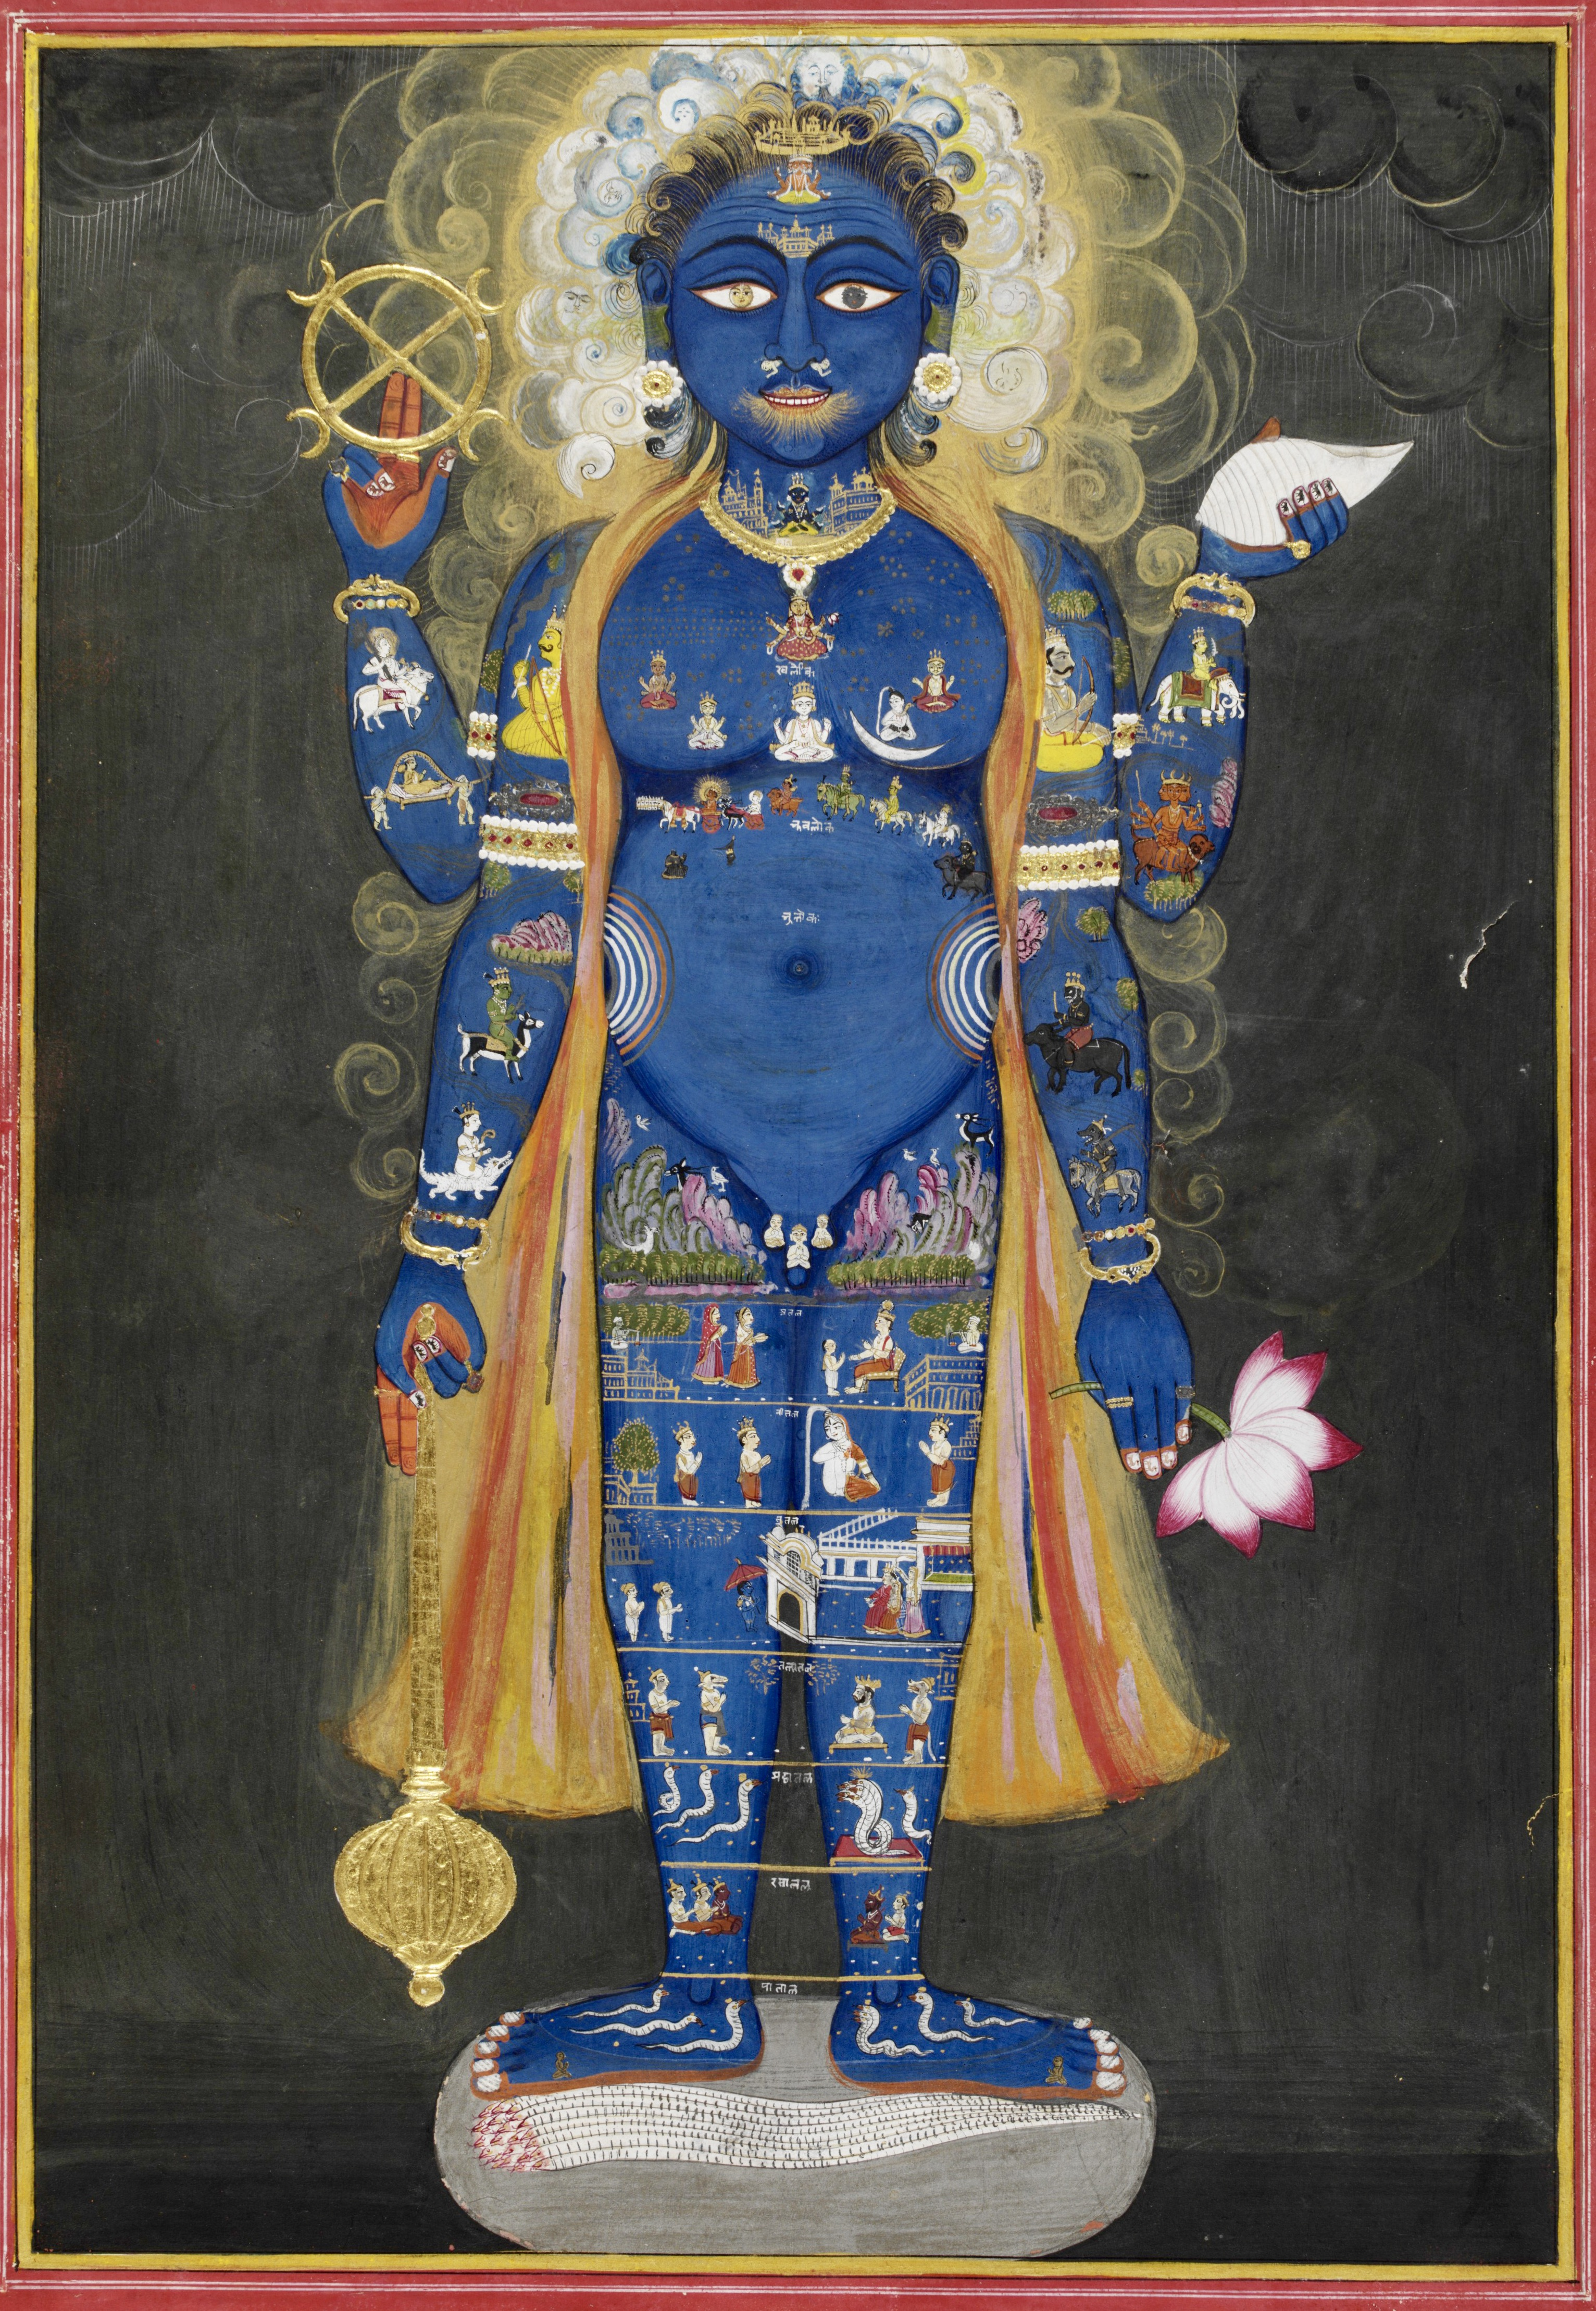
\includegraphics[width=1\textwidth]{pics/Vishnu_Vishvarupa_cropped.jpg}
	\caption{Viṣṇu Viśvarūpa, India, Rajasthan, Jaipur, ca. 1800–1820, Opaque watercolor and gold on paper, 38.5 × 28 cm, Victoria and Albert Museum, London, Given by Mrs. Gerald Clark.}
	\label{fig1}
      \end{figure}
\clearpage
  \begin{figure}[ht]
	\centering
  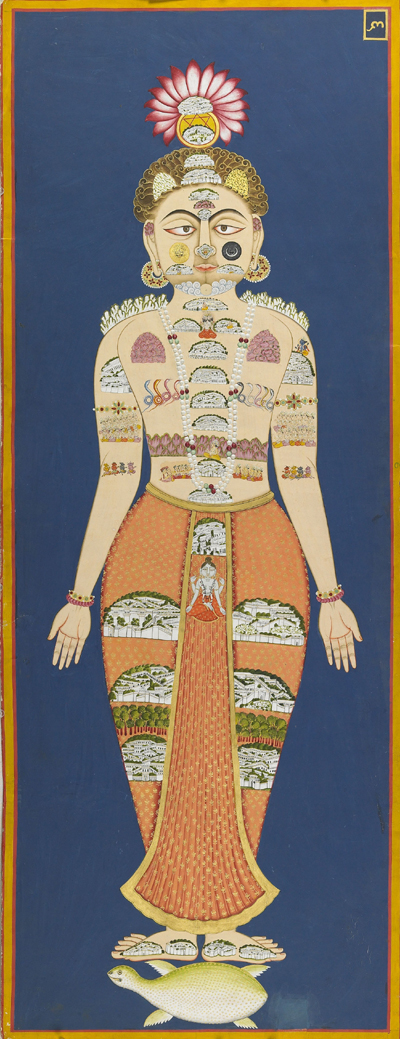
\includegraphics[width=0.5\textwidth]{pics/The_Equivalence_of_Self_and_Universe_(detail),_folio_6_from_the_Siddha_Siddhanta_Paddhati,_(Bulaki),_1824_(Samvat_1881);_122_x_46_cm._Mehrangarh_Museum_Trust..jpg}
	\caption{The Equivalence of Self and Universe (detail), folio 6 from the \textit{Siddhasiddhāntapaddhati} (Bulaki), India, Rajasthan, Jodhpur, 1824 (Samvat 1881), 122 x 46 cm, RJS 2378, Mehragarh Museum Trust.}
	\label{fig2}
      \end{figure}
      % \end{landscape}


\chapter{Bibliography}
 \label{sec:bibli}
   \clearpage
\newpage 
\thispagestyle{empty}
\quad  \addtocounter{page}{-1}

\printbibliography[heading=subbibintoc, title=Consulted Manuscripts, keyword=codex]

\printbibliography[heading=subbibintoc, title=Printed Editions, keyword=printsource]

\printbibliography[heading=subbibintoc, title=Secondary Literature, keyword=seclit]

\printbibliography[heading=subbibintoc, title=Online Sources, keyword=onlinesource]

\end{document}
